
\documentclass{beamer}

\usepackage[style=authoryear]{biblatex}
\usepackage{ragged2e}
\definecolor{links}{HTML}{0366d6}
\definecolor{cite_color}{HTML}{000000}
\hypersetup{colorlinks,linkcolor=,urlcolor=links,citecolor=cite_color}
\usepackage{graphicx,ru,url}
\usepackage[brazilian]{babel}
\usepackage[utf8]{inputenc}
\usepackage{graphicx}
\usepackage{epstopdf}
\usepackage{listings}
\usepackage{dirtree}
\usepackage{colortbl}
\usepackage{upquote}
\usepackage{csquotes}

\setbeamertemplate{caption}[numbered]
\setbeamercolor*{bibliography entry title}{fg=black}
\setbeamercolor*{bibliography entry location}{fg=black}
\setbeamercolor*{bibliography entry note}{fg=black}
\setbeamertemplate{bibliography item}{}
\renewcommand*{\bibfont}{\tiny}
\renewcommand*{\nameyeardelim}{\addcomma\addspace}

\addbibresource{bibliografia.bib}

%\include{defs}

\usepackage{float} %imagem e tabelas
\usepackage{booktabs} %tabelas	

\epstopdfDeclareGraphicsRule{.gif}{png}{.png}{convert gif:#1 png:\OutputFile}
\AppendGraphicsExtensions{.gif}

% The title of the presentation:
%  - first a short version which is visible at the bottom of each slide;
%  - second the full title shown on the title slide;
\title[Apresentação TCC II]{Um sistema computacional capaz de determinar o potencial energético solar de um estabelecimento ou residência}

% The author(s) of the presentation:
%  - again first a short version to be displayed at the bottom;
%  - next the full list of authors, which may include contact information;
\author[Felipe Leon]{
 \texorpdfstring{Felipe Garcia de Leon\\}{}
 \href{mailto:felipe.deleon@yahoo.com.br}{felipe.deleon@yahoo.com.br}
}
 
% The institute:
%  - to start the name of the university as displayed on the top of each slide
%    this can be adjusted such that you can also create a Dutch version
%  - next the institute information as displayed on the title slide
\institute[Universidade Federal de Pelotas]{}

% Add a date and possibly the name of the event to the slides
%  - again first a short version to be shown at the bottom of each slide
%  - second the full date and event name for the title slide
\date[Pelotas - Dezembro 2021]{
  Orientador: Prof. Dr. Eng. Cláudio Manoel da Cunha Duarte
  Pelotas, 2021
}

\begin{document}

\begin{frame}
  \titlepage
\end{frame}

%===================================================================

\begin{frame}
  \frametitle{Sumário}

  \tableofcontents
\end{frame}
%=================================================================
\AtBeginSection[]
{
\begin{frame}
\frametitle{Sumário}
\tableofcontents[currentsection]
\end{frame}
}


%===================================================================
\section{Introdução}

\begin{frame}

\begin{figure}[H]
    \centering
    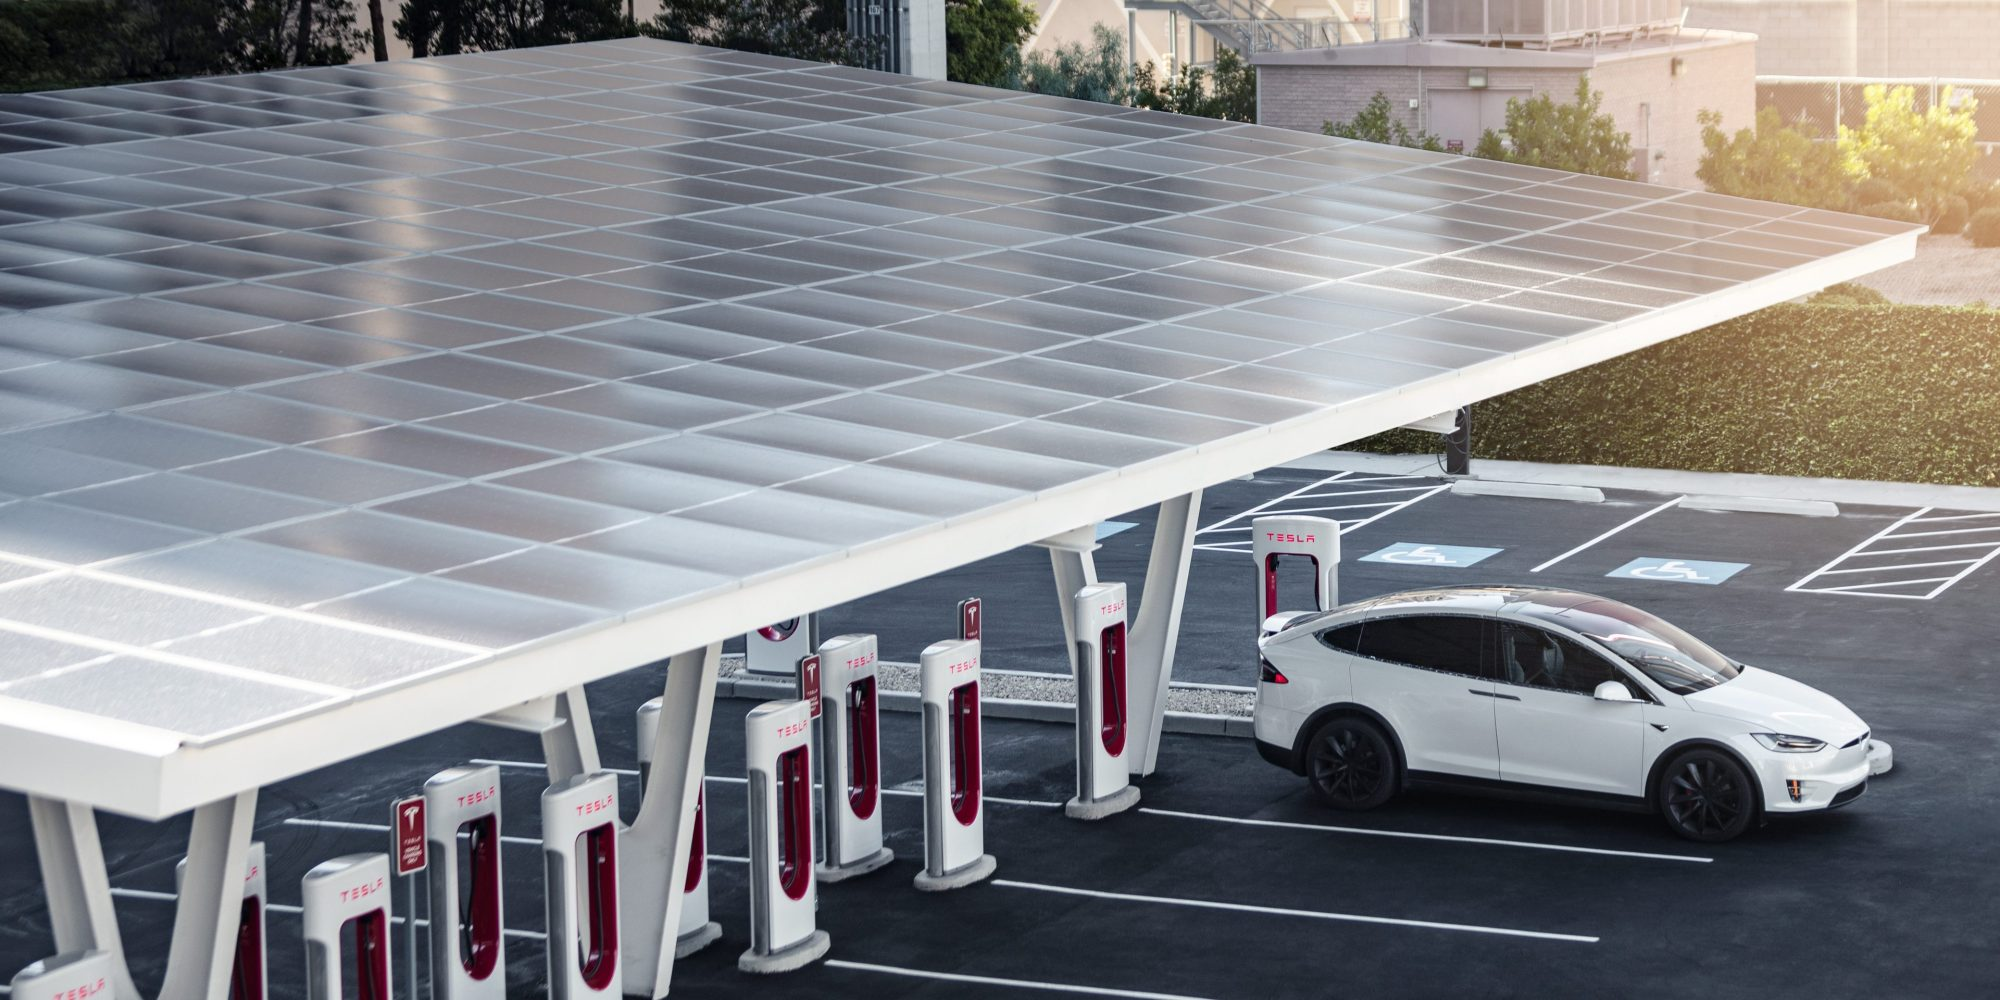
\includegraphics[width=0.95\textwidth]{./Figuras/vegas_charge.jpeg}
    \caption{Estação de recarga V3 Supercharging em Las Vegas (USA).}{Fonte: \cite{tesla}}
   \label{fig:tesla_charge}
\end{figure}

\end{frame}

\begin{frame}{Objetivo}

  \begin{itemize}
  
    \item Desenvolver um modelo matemático capaz de determinar custos e retornos assim como a capacidade de produção de energia elétrica de um sistema fotovoltaico, utilizado como cogerador de energia para uma estação de recarga veicular;
    
    \item Desenvolver e publicar um aplicativo acessível através da internet capaz de ser usado para demonstrar os resultados do modelo desenvolvido;
    
    \item Utilizar o aplicativo para demonstrar os resultados relativos à produção de energia, custos e retornos financeiros e aos benefícios do sistema.
      
  \end{itemize}

\end{frame}

%============================================================

\section{Revisão bibliográfica}

%--------------------

\begin{frame}{Energia solar}

 A energia irradiada pelo Sol cobre uma ampla faixa do espectro eletromagnético, conforme ilustra a Figura \ref{fig:irrad_solar}. Cerca de 81\% da energia que chega ao Sistema Terra/Atmosfera está em uma faixa de comprimentos de onda que vai do visível ao infravermelho próximo \cite{atlas2017}.
 
\begin{figure}[H]
    \centering
    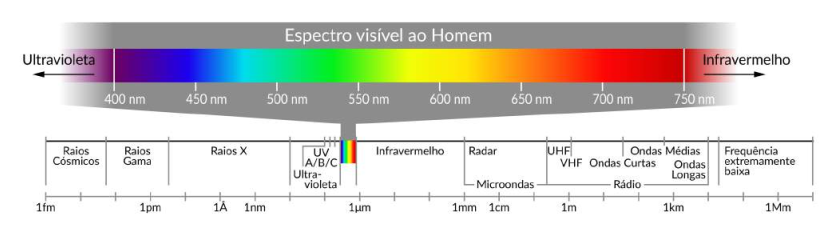
\includegraphics[width=0.9\textwidth]{./Figuras/irrad_solar.png}
    \caption{Espectro da radiação solar incluindo um detalhamento da faixa visível humana.}{Fonte: \cite{atlas2017}}
   \label{fig:irrad_solar}
\end{figure}

\end{frame}

%--------------------

\begin{frame}{Sistema de energia solar moderno}

\begin{figure}[ht]
    \centering
    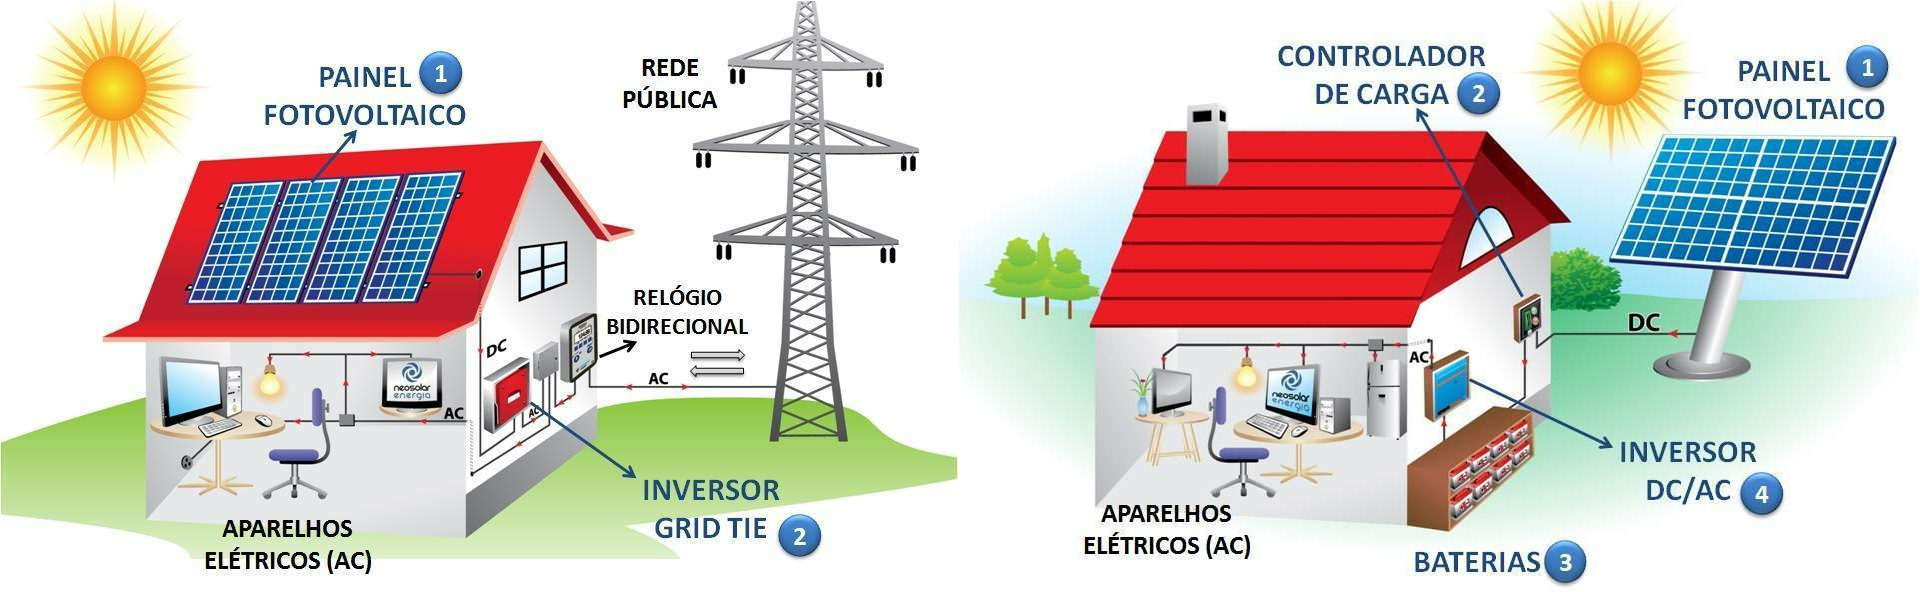
\includegraphics[width=0.985\textwidth]{./Figuras/sistemas_pv.png}
    \caption{Painel residencial solar conectado à rede e off-grid respectivamente.}{Fonte: \cite{neosolar}}
   \label{fig:sistema_pv_rede}
\end{figure}

\end{frame}

%--------------------

\begin{frame}{Dispositivos fotovoltaicos (PV)}

O efeito PV foi observado já em 1839 por Alexandre Edmund Becquerel e foi objeto de investigação científica ao longo do início do século XX. 

\begin{figure}[ht]
    \centering
    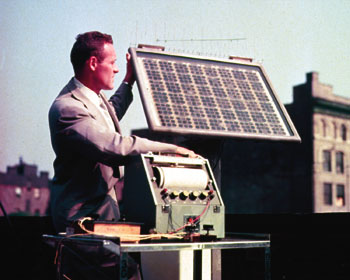
\includegraphics[width=0.4\textwidth]{./Figuras/1954_solar2.jpg}
    \caption{Engenheiro da Bell Labs testando bateria solar em 1954, o primeiro dispositivo solar fotovoltaico.}{Fonte: \cite{belllabs_photovoltaics}}
   \label{fig:1954_solar2}
\end{figure}

\end{frame}

%--------------------

\begin{frame}{Dispositivos fotovoltaicos modernos   }

\begin{figure}[ht]
    \centering
    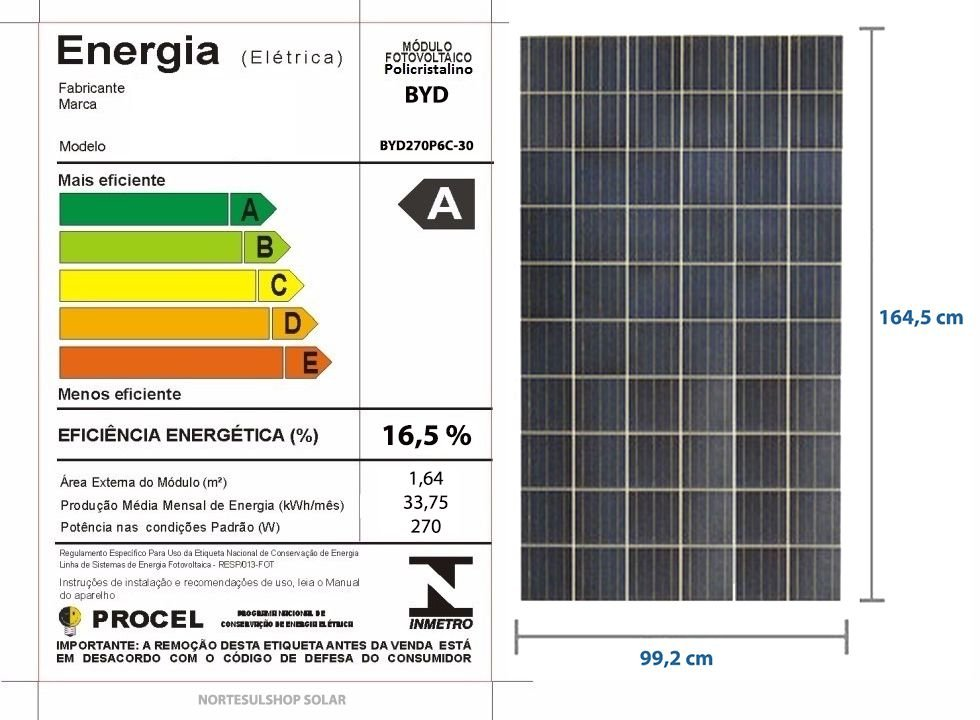
\includegraphics[width=0.5\textwidth]{./Figuras/BYD270P6C.jpg}
    \caption{Painel fotovoltaico moderno modelo BYD270P6C-30.}{Fonte: \cite{nortesulshop}}
   \label{fig:BYD270P6C}
\end{figure}

\end{frame}

%--------------------

\begin{frame}{Célula fotovoltaica}

\begin{figure}[ht]
    \centering
    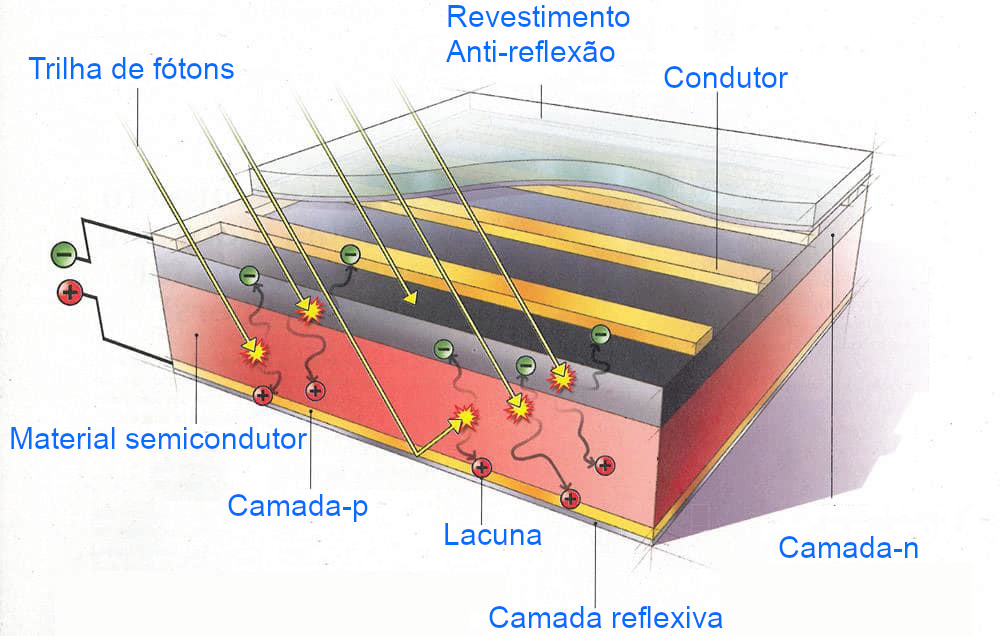
\includegraphics[width=0.5\textwidth]{./Figuras/pv-cell.jpg}
    \caption{Diagrama de uma típica célula solar de silício cristalino. Para fazer esse tipo de célula, wafers de silício de alta pureza são “dopados” com várias impurezas e fundidos. A estrutura resultante cria um caminho para a corrente elétrica dentro e entre as células solares.}{Fonte: \cite{seia}}
   \label{fig:pv-cell}
\end{figure}

\end{frame}

%--------------------

\begin{frame}{Eficiência e potência de painéis solares}

\begin{figure}[H]
    \centering
    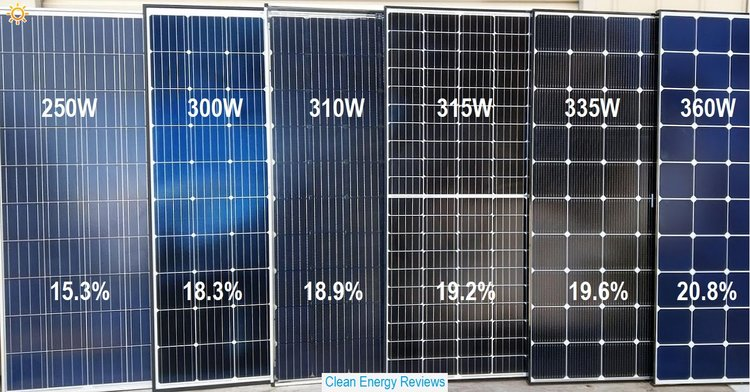
\includegraphics[width=0.8\textwidth]{./Figuras/pvs_pot.jpg}
    \caption{Eficiência e potência em relação ao tipo de painel.}{Fonte: \cite{cleanenergyreviews}}
   \label{fig:pvs_pot}
\end{figure}

\end{frame}

%--------------------

\begin{frame}{Eficiência em relação ao tamanho}

\begin{figure}[H]
    \centering
    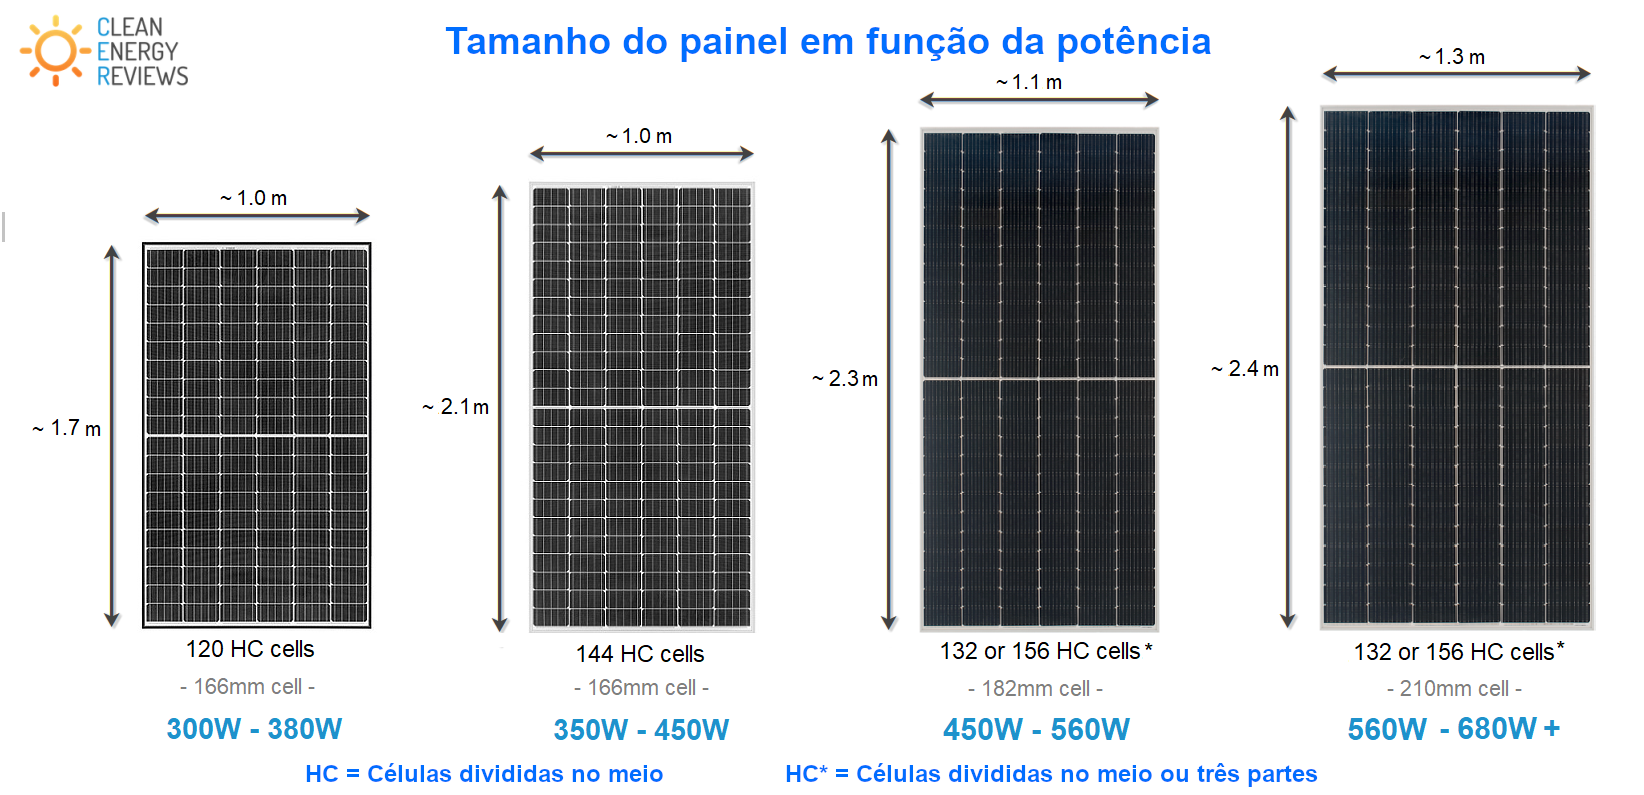
\includegraphics[width=0.975\textwidth]{./Figuras/pv_size.png}
    \caption{Tamanho do painel em função da potência.}{Fonte: \cite{cleanenergyreviews}}
   \label{fig:pv_size}
\end{figure}

\end{frame}

%--------------------

\begin{frame}{Desempenho de operação painéis solares}

Os valores nominais de eficiência e potência, descrevem o desempenho do painel quando em operação ideal, mas no mundo real temos muitos fatores que influenciam essa operação tais como:

\begin{itemize}
  \item Irradiância solar em W/m².

  \item Temperatura do painel.
  
  \item Sombras.
  
  \item Orientação do painel.
  
  \item Localização (latitude).
  
  \item Época do ano.
  
  \item Sujeira sobre o painel.
\end{itemize}

\end{frame}

%--------------------

\begin{frame}{Desempenho de operação painéis solares}

Os dois principais fatores que afetam o desempenho são Irradiância solar em W/m² e Temperatura. A redução da irradiação que chega ao painel diminui a sua capacidade de produzir energia.

\begin{figure}[H]
    \centering
    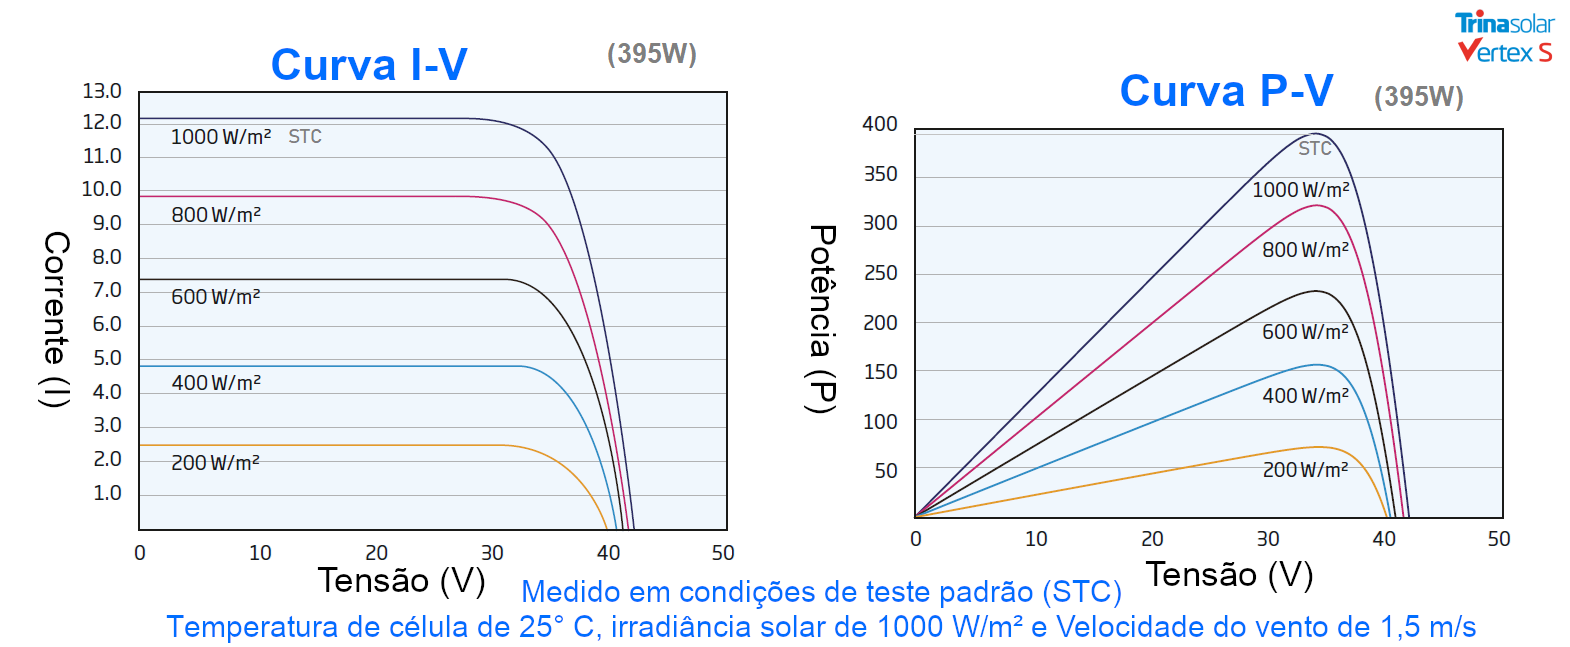
\includegraphics[width=0.775\textwidth]{./Figuras/pv_luz.png}
    \caption{Curvas de desempenho em relação à Irradiância solar.}{Fonte: \cite{cleanenergyreviews}}
   \label{fig:pv_luz}
\end{figure}

\end{frame}

%--------------------

\begin{frame}{Desempenho de operação painéis solares}

\begin{figure}[H]
    \centering
    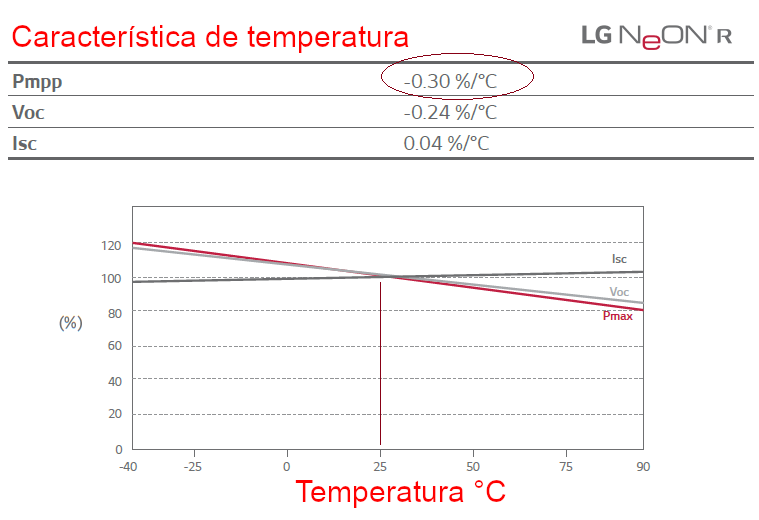
\includegraphics[width=0.7\textwidth]{./Figuras/pv_temp.png}
    \caption{Perda de potência máxima em função da temperatura.}{Fonte: \cite{LG350Q1C}}
   \label{fig:pv_temp}
\end{figure}

\end{frame}

%--------------------

\begin{frame}{Inversores e otimizador de potência}

\begin{figure}[ht]
    \centering
    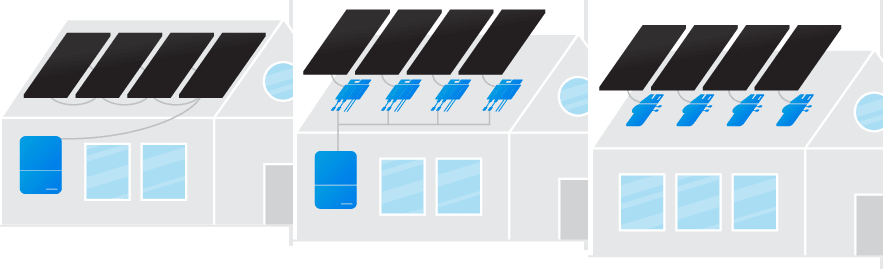
\includegraphics[width=0.95\textwidth]{./Figuras/inv_opt.png}
    \caption{Inversores e otimizador de potência}{Fonte: \cite{EnergySage}}
   \label{fig:opt}
\end{figure}

\end{frame}

%--------------------

\begin{frame}{Panorama elétrico nacional}

Todos os meses, a ANEEL/ABSOLAR \cite{ABSOLAR} analisa e consolida dados do setor e produz um infográfico com o cenário da energia solar PV no País, a partir desse infográfico é possível extrair o panorama nacional elétrico, conforme descrito a seguir.

\end{frame}

%--------------------

\begin{frame}{Matriz elétrica Brasileira}

\begin{figure}[H]
    \centering
    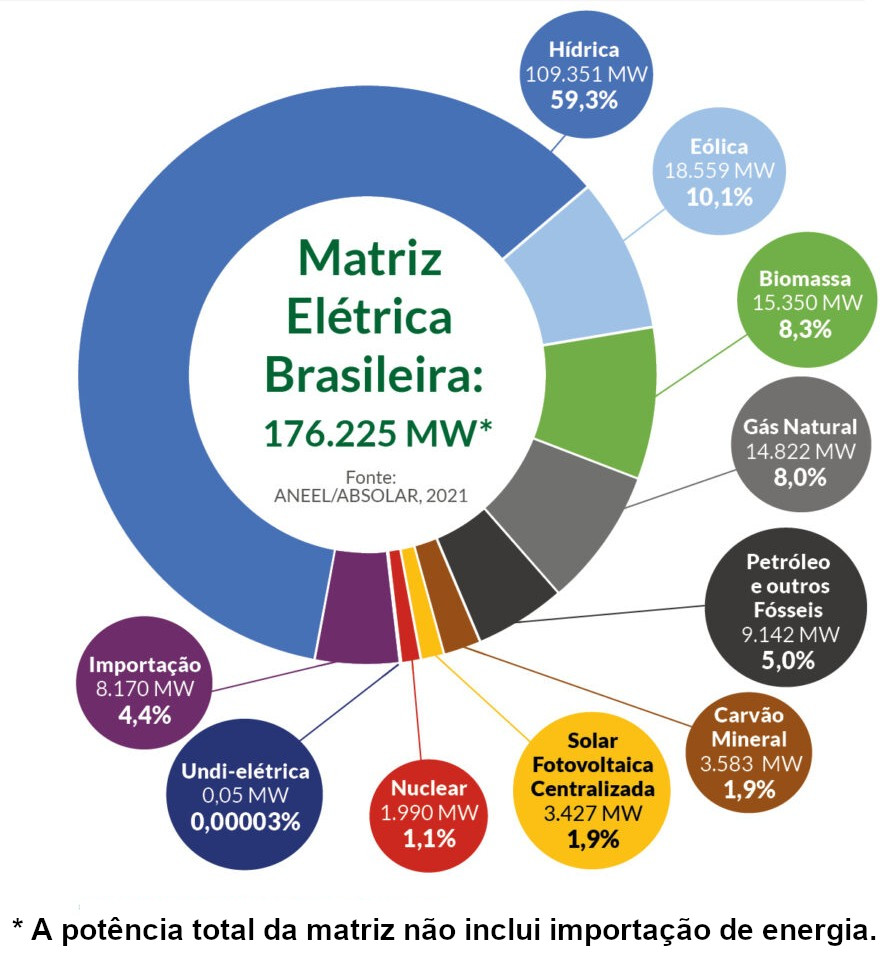
\includegraphics[width=0.4\textwidth]{./Figuras/mz_brasil.jpg}
    \caption{Matriz elétrica brasileira.}{Fonte: \cite{ABSOLAR}}
   \label{fig:mz_brasil}
\end{figure}

Energia hídrica 59,3\%, eólica 10,1\% e solar 1,9\% somam 71,3\%.

\end{frame}

%--------------------

\begin{frame}{Evolução do uso da energia solar fotovoltaica no Brasil}

\begin{figure}[H]
    \centering
    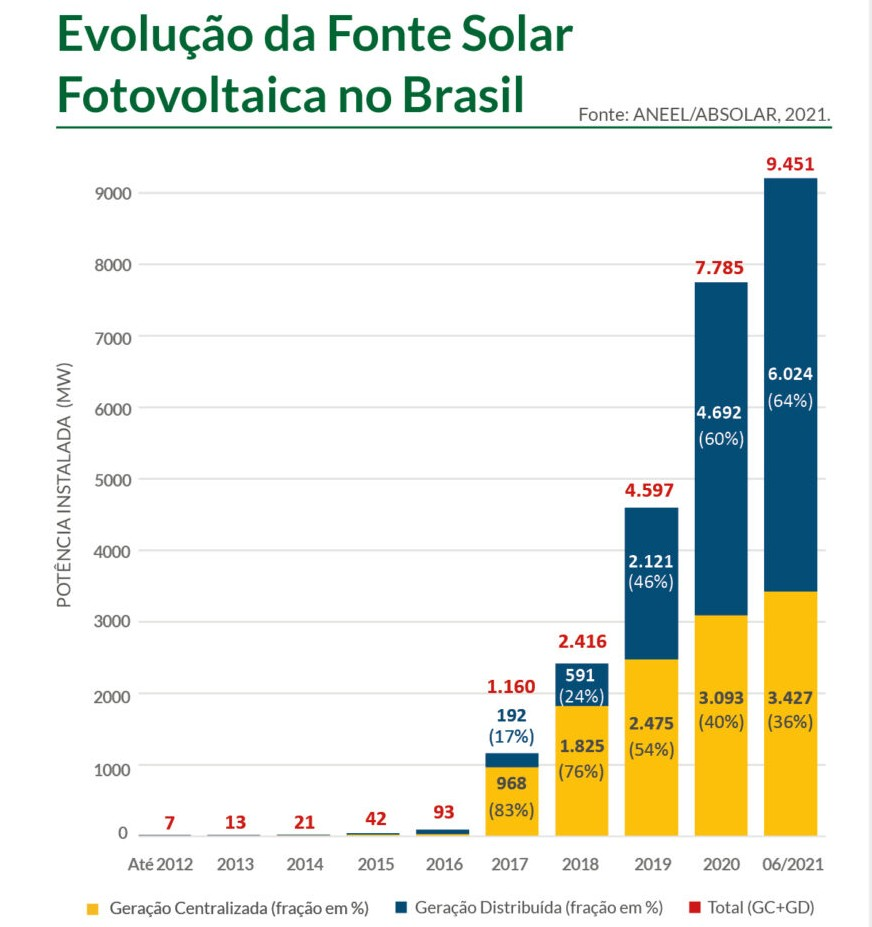
\includegraphics[width=0.425\textwidth]{./Figuras/ev_solar.jpg}
    \caption{Evolução da fonte solar fotovoltaica no Brasil.}{Fonte: \cite{ABSOLAR}}
   \label{fig:ev_solar}
\end{figure}

\end{frame}

%--------------------

\begin{frame}{Potencial solar brasileiro}

\begin{figure}[H]
    \centering
    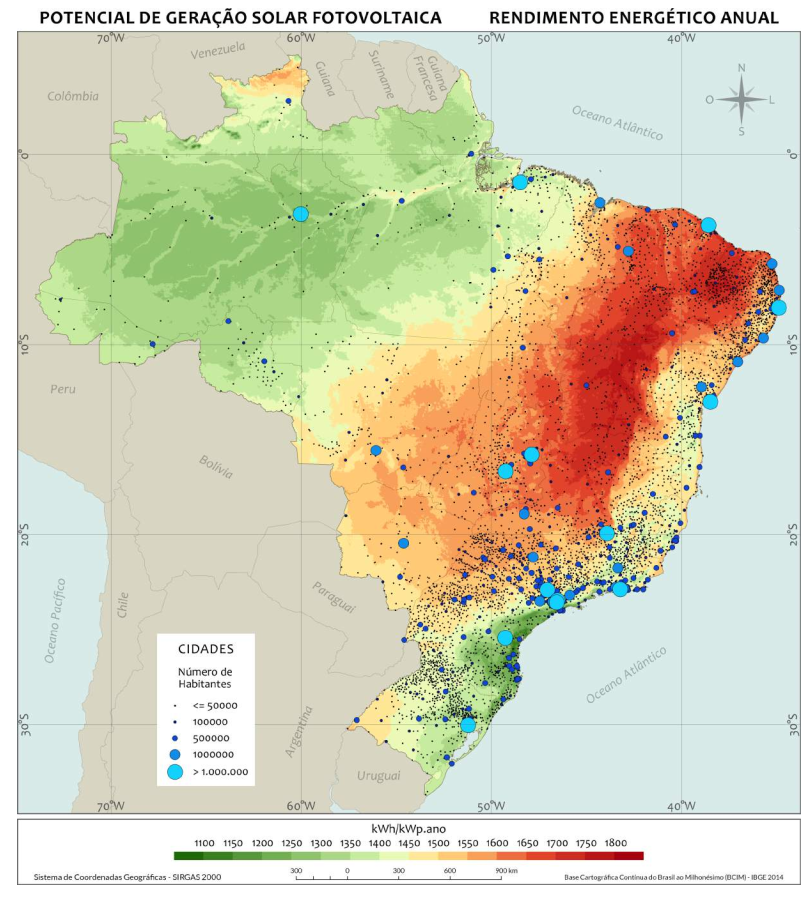
\includegraphics[width=0.3\textwidth]{./Figuras/pot_geracao_solar.png}
    \caption{Mapa do potencial de geração solar fotovoltaica em termos do rendimento energético anual para todo o Brasil (medido em kWh/kWp.ano no perfil de cores), admitindo uma taxa de desempenho de 80\% para geradores fotovoltaicos fixos e distribuição da população brasileira nas cidades.}{Fonte: \cite{atlas2017}}
   \label{fig:pot_geracao_solar}
\end{figure}

\end{frame}

%--------------------

\begin{frame}{Custo da energia elétrica no Brasil}

\begin{figure}[H]
    \centering
    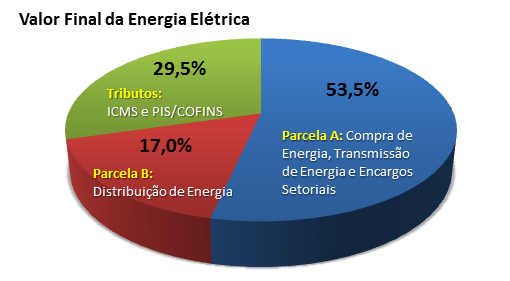
\includegraphics[width=0.85\textwidth]{./Figuras/valor_tarifa.png}
    \caption{Valor final da energia elétrica.}{Fonte: \cite{ANEEL_TARIFA}}
   \label{fig:valor_tarifa}
\end{figure}

\end{frame}

%--------------------

\begin{frame}{Custo final kWh cobrado pela CEEE}

O custo por kWh real cobrado pela CEEE é descrito na Tabela \ref{kwh_ceee}. Sendo o valor base do kWh (R\$ 0,54897) usado pela distribuidora.

\begin{table}[htbp]
    \caption{Custo final kWh cobrado pela CEEE.}
        \begin{center}
            \begin{tabular}{ >{\centering\arraybackslash} m{3cm} >{\centering\arraybackslash} m{7cm}  }
                \hline
                Bandeira & Custo kWh \newline (já com todos tributos acréscimo de 50,8\%) \\ \hline
                Verde & R\$ 0,82857\\
                Amarela & R\$ 0,84882 \\
                Vermelha 1 & R\$ 0,89143\\
                Vermelha 2 & R\$ 0,92270 \\ \hline
            \end{tabular}
        \end{center}
    \label{kwh_ceee}
\end{table}

O custo final pode chegar a ser R\$ 0,9227 o kWh,\newline um valor 68,08 \% maior que o valor base do kWh.

\end{frame}

%--------------------

\begin{frame}{Determinando o potencial energético de uma região }

Para que seja possível quantificar o quanto uma região pode gerar anualmente de energia solar, primeiro é preciso compreender os diversos fatores que influenciam esse sistema na prática.
\newline
\newline
Anteriormente foram definidos os principais fatores que influenciam a desempenho dos painéis solares, como, \textbf{irradiância solar, temperatura do painel, sombras, orientação e etc}. A seguir, serão definidos os fatores práticos relacionando \textbf{geografia, meteorologia e componentes da irradiação} que são usados para determinar e ou prever os fatores da seção anterior.

\end{frame}

%--------------------

\begin{frame}{Posição relativa entre o Sol e a Terra}

\begin{figure}[H]
    \centering
    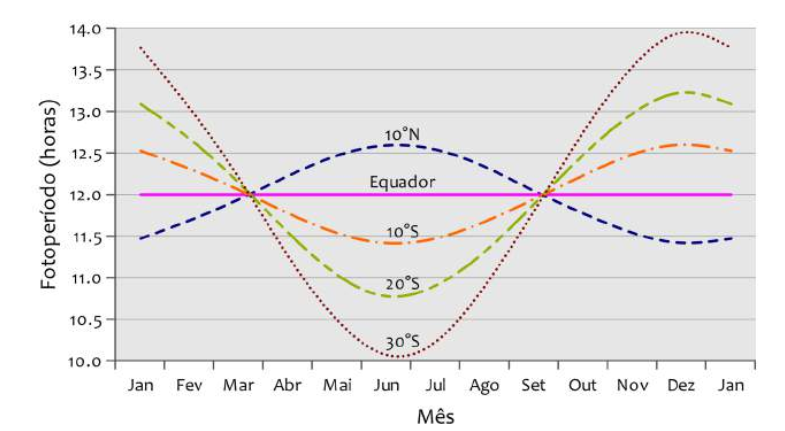
\includegraphics[width=0.75\textwidth]{./Figuras/dia_luz.png}
    \caption{Variabilidade do fotoperíodo ao longo do ano para diferentes latitudes. Deve‐se notar que o fotoperíodo apresenta maior variabilidade à medida que a localidade está mais próxima dos polos.}{Fonte: \cite{atlas2017}}
   \label{fig:dia_luz}
\end{figure}

\end{frame}

%--------------------

\begin{frame}{Meteorologia para produção de energia}


A disponibilidade e a variabilidade dos recursos energéticos estão intrinsecamente associados às condições do clima da região. Isso ocorre porque sistemas meteorológicos provocam alterações na nebulosidade e nas concentrações dos gases e aerossóis, afetando os processos radiativos que atenuam a radiação solar ao longo de seu percurso na atmosfera.

\end{frame}

%--------------------

\begin{frame}{Valores médios anuais de precipitação observados no território brasileiro}

\begin{figure}[H]
    \centering
    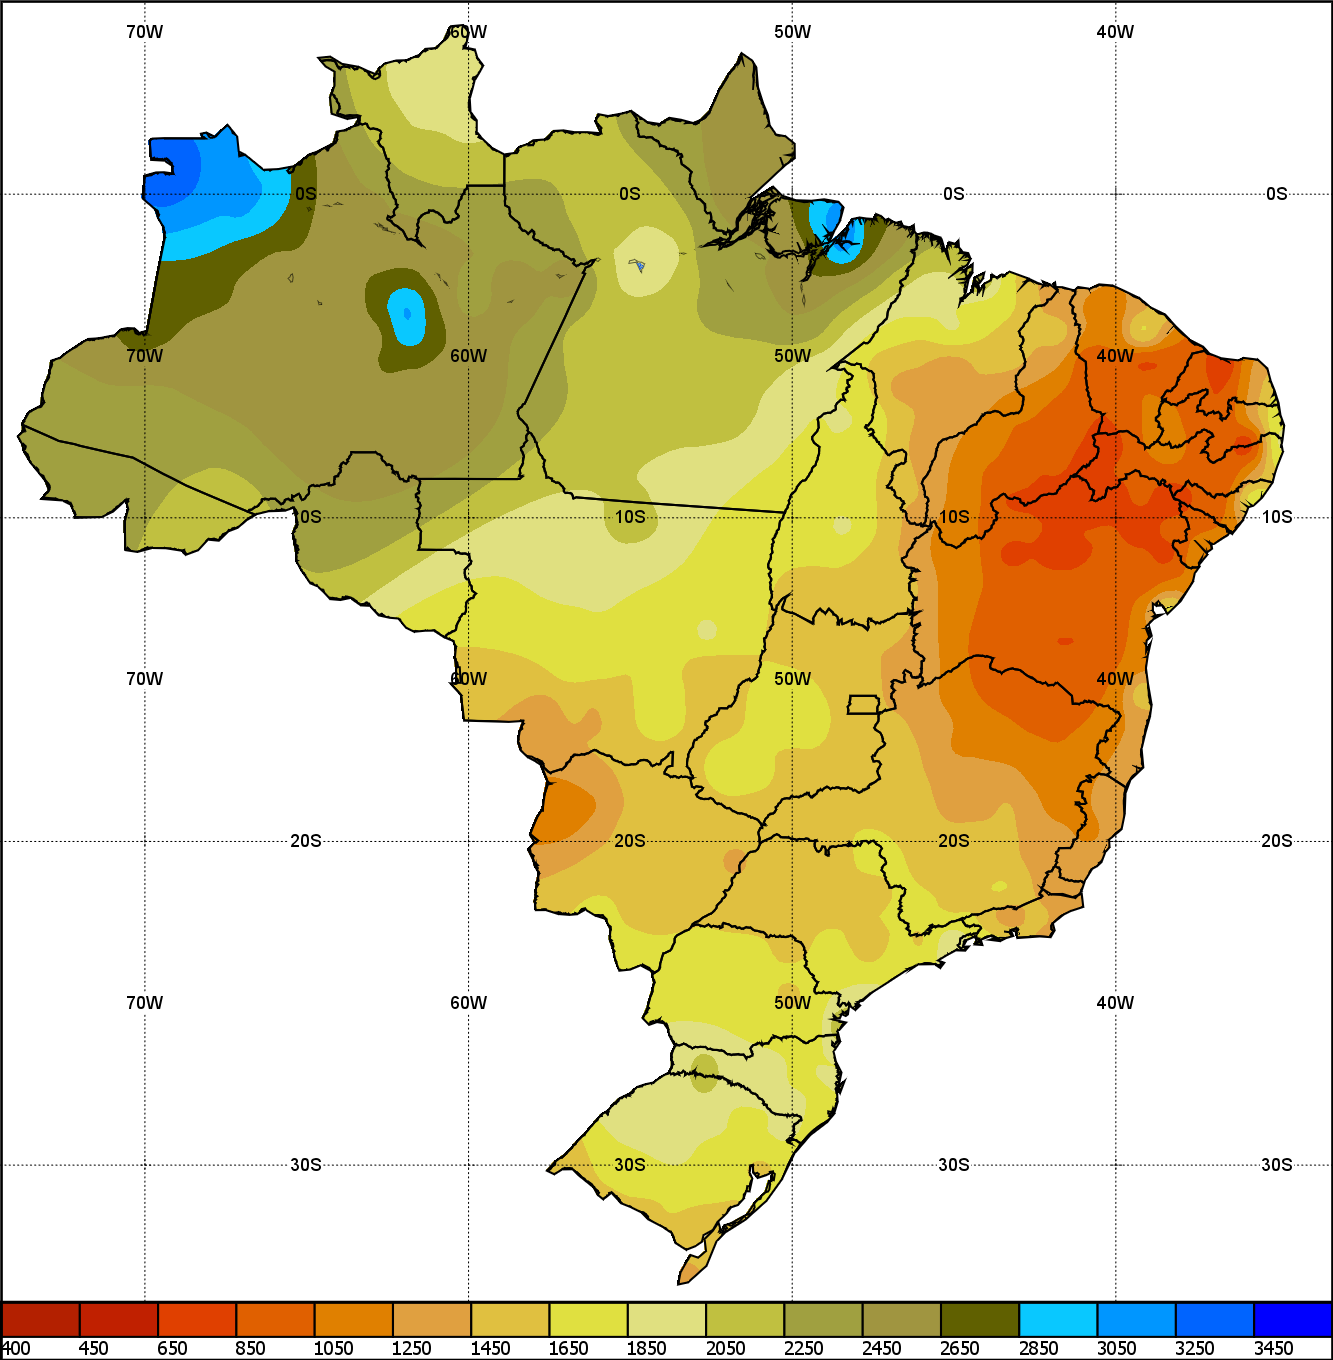
\includegraphics[width=0.4\textwidth]{./Figuras/chuvas_clima.png}
    \caption{Normal climatológica (1981‐2010)  de precipitação anual.}{Fonte: \cite{INMET}}
   \label{fig:chuvas_clima}
\end{figure}

\end{frame}

%--------------------

\begin{frame}{Temperaturas médias no território brasileiro}

\begin{figure}[H]
    \centering
    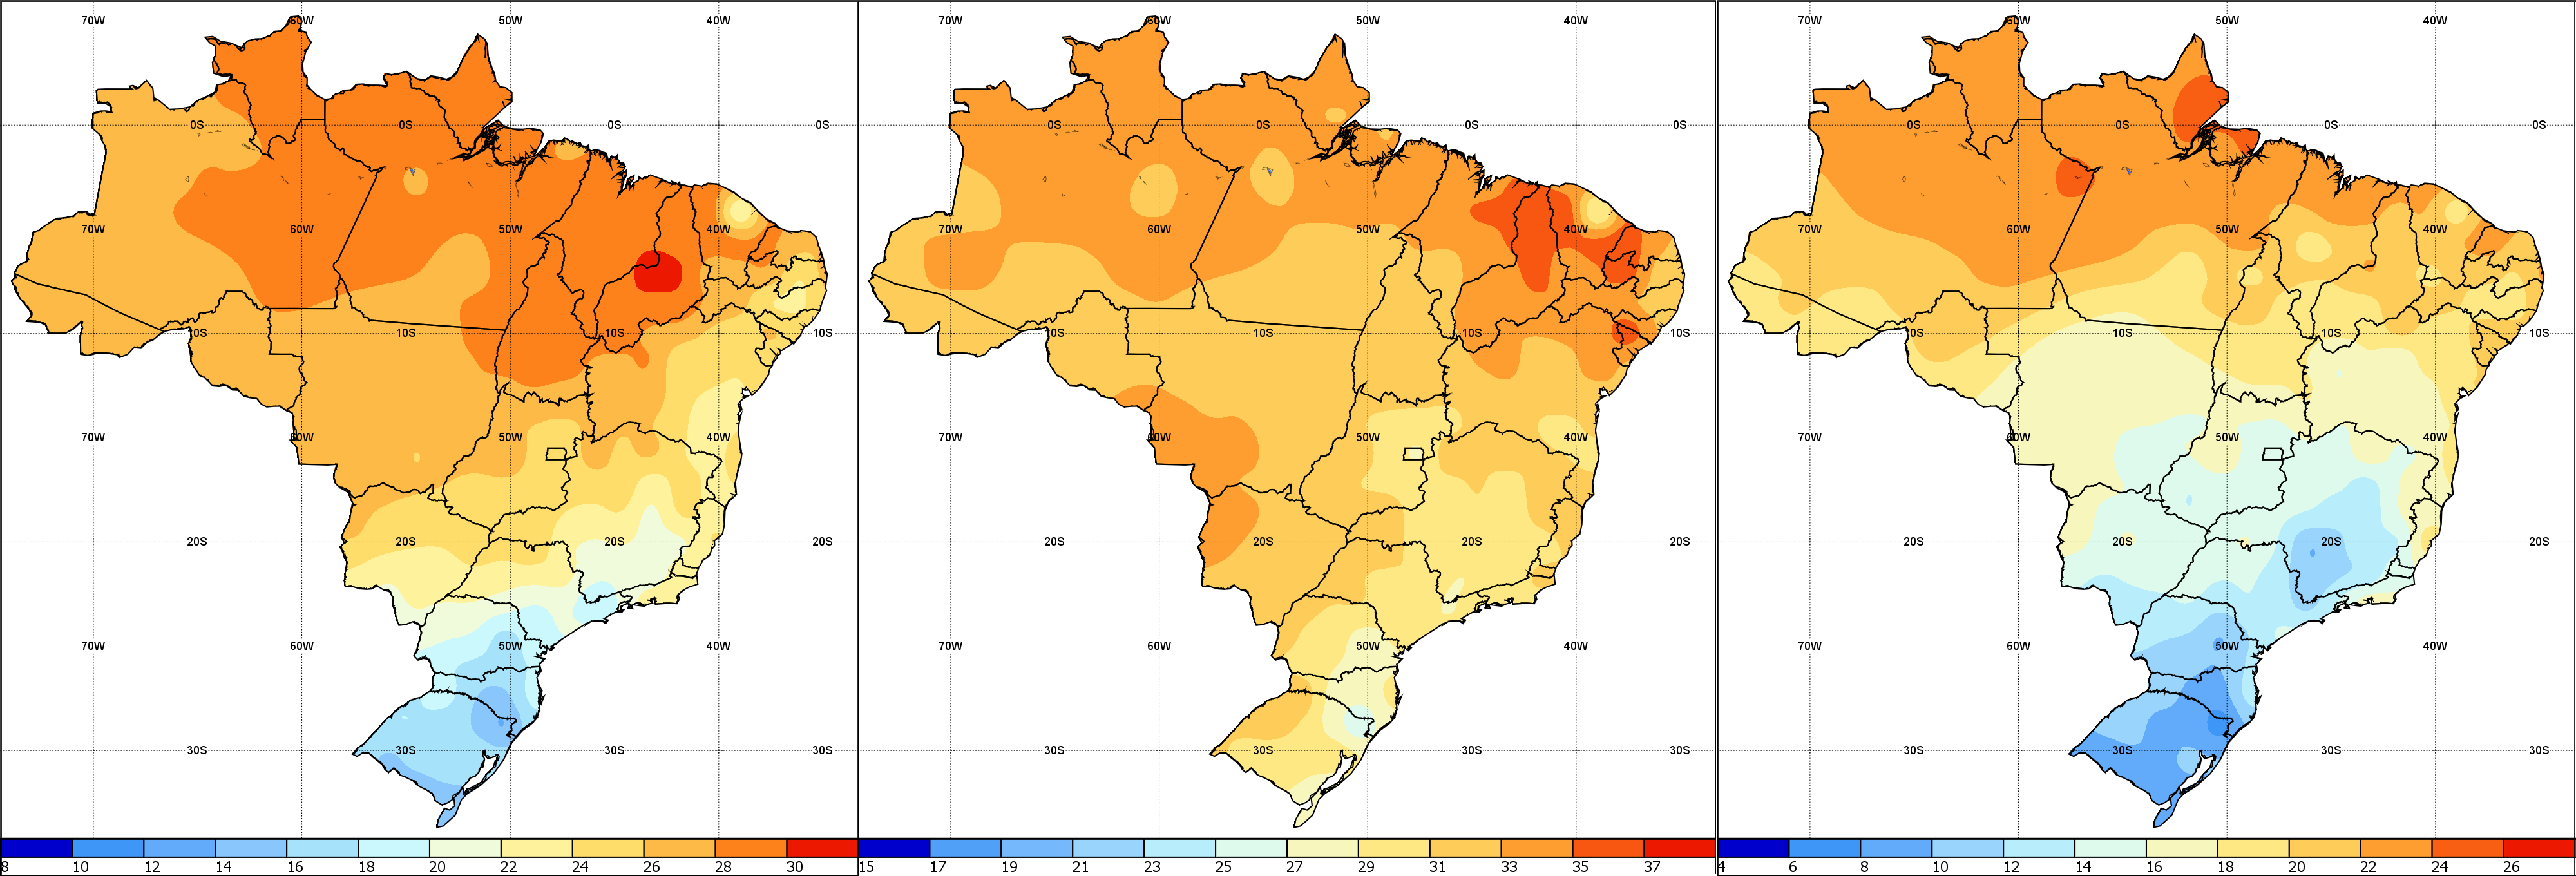
\includegraphics[width=0.95\textwidth]{./Figuras/temperatura_clima.png}
    \caption{ Normais climatológicas (1981‐2010) de temperatura no território brasileiro: (a) média anual dos valores de temperatura; (b) média de temperatura máxima observada no mês de dezembro; e (c) média de temperatura mínima observada no mês de junho.}{Fonte: \cite{INMET}}
   \label{fig:temperatura_clima}
\end{figure}

\end{frame}

%--------------------

\begin{frame}{Instrumentação e aquisição de dados}

\textbf{Piranômetro de termopilha}

\begin{figure}[H]
    \centering
    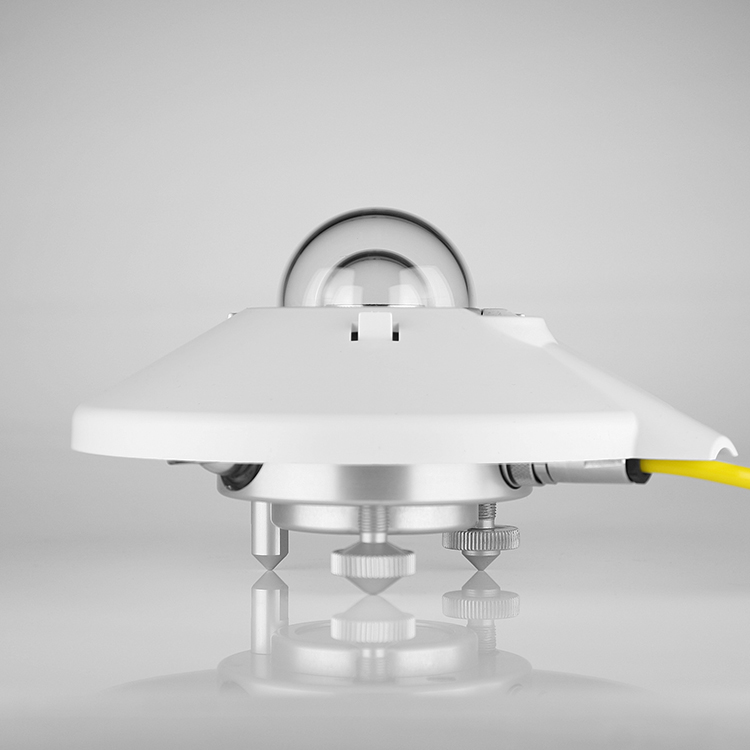
\includegraphics[width=0.4\textwidth]{./Figuras/pirometro_termo.jpg}
    \caption{ Piranômetro de fotodiodo de termopilha.}{Fonte: \cite{kippzonen}}
   \label{fig:pirometro_termo}
\end{figure}

\end{frame}

%--------------------

\begin{frame}{Pireliômetro}

\begin{figure}[H]
    \centering
    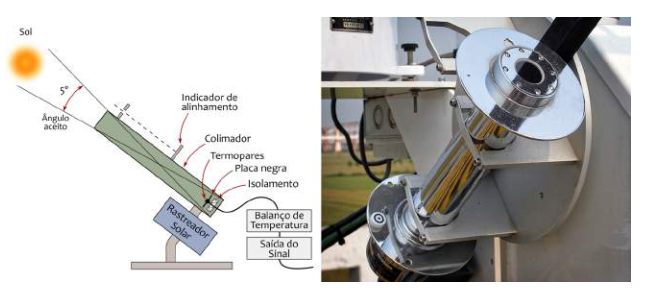
\includegraphics[width=0.95\textwidth]{./Figuras/pirheliometro.png}
    \caption{Representação gráfica e imagem de um pireliômetro.}{Fonte: \cite{kippzonen}}
   \label{fig:pirheliometro}
\end{figure}

\end{frame}


%--------------------

\begin{frame}{Sistemas de sombreamento}

\begin{figure}[H]
    \centering
    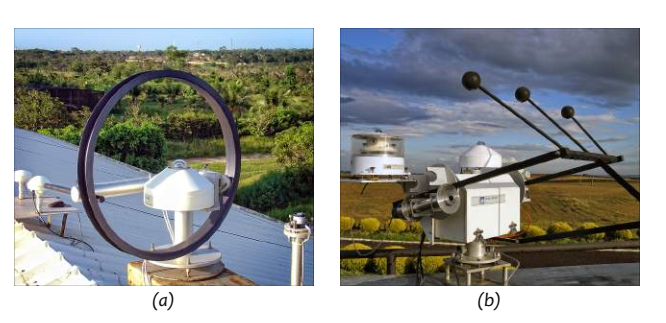
\includegraphics[width=0.8\textwidth]{./Figuras/sis_sombra.png}
    \caption{Sistemas para sombreamento do piranômetro utilizados na aquisição de dados de radiação difusa: anel de sombreamento (a) e esfera de sombreamento com rastreador solar (b).}{Fonte: \cite{atlas2017}}
   \label{fig:sis_sombra}
\end{figure}

\end{frame}

%--------------------

\begin{frame}{Estações meteorológicas automáticas do INMET}

\begin{figure}[H]
    \centering
    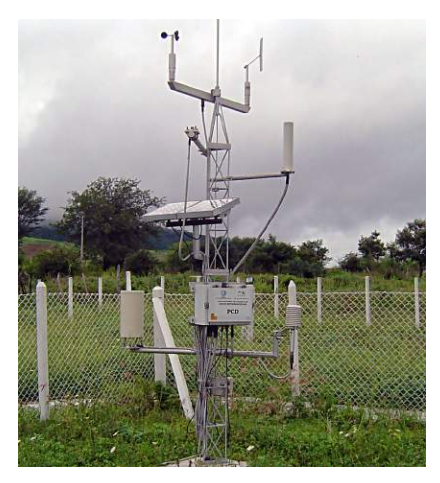
\includegraphics[width=0.4\textwidth]{./Figuras/estacao_meteorologicas.png}
    \caption{Foto de estação automática de coleta de dados.}{Fonte: \cite{atlas2017}}
   \label{fig:estacao_meteorologicas}
\end{figure}


\end{frame}

%--------------------

\begin{frame}{Modelagem de sistemas de energia fotovoltaica}

Para o desenvolvimento deste projeto escolheu-se utilizar um modelo matemático para determinar a performance de um sistema PV. O laboratório nacional (EUA) Sandia desenvolveu uma biblioteca de livre acesso que permite modelar todos o processo de um sistema PV.

\begin{figure}[H]
    \centering
    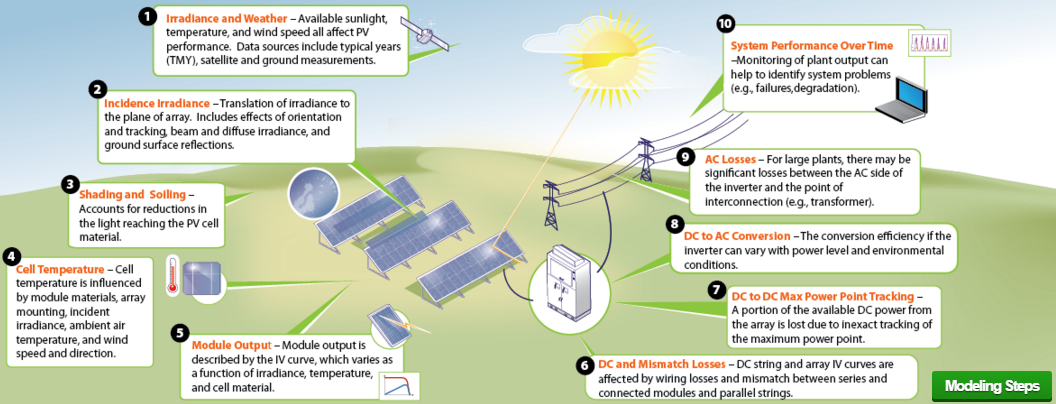
\includegraphics[width=0.7\textwidth]{./Figuras/sandia_model.png}
    \caption{Modelo PV PMC do Sandia.}{Fonte: \cite{sandia}}
   \label{fig:sandia_model}
\end{figure}

\end{frame}


%--------------------

\begin{frame}{Equações do modelo}

\begin{itemize}
  \item Irradiância incidente no plano da matriz (POA).
  
  \item Temperatura do modulo.

  \item Temperatura da célula.
  
  \item Potência máxima CC.
  
   \item Conversão CC-CA.
   
   \item Perdas.
   
   \item Etc...
\end{itemize}

\end{frame}

%--------------------

\begin{frame}{}

\tiny
\begin{table}[htbp]
    \caption{Tabela dados dos veículos mais vendidos Brasil 2020}
        \begin{center}
            \begin{tabular}{ >{\centering\arraybackslash} m{3cm} >{\centering\arraybackslash} m{2cm} >{\centering\arraybackslash} m{1cm} >{\centering\arraybackslash} m{2cm} }
                \hline
                Modelo (Montadora) & Bateria & Autonomia & Velocidade de Recarga 80 \% \\ \hline %Primeira e ultima linha adiciona \hline apos \\
                E-TRON \cite{E-TRON} &  95 kWh 396 V & 436 km & 30 m 150 kW \\
                BOLT \cite{BOLT} & 60 kWh 120 V & 416 km & 1 h 55 kW \\
                LEAF  \cite{LEAF} & 40 kWh 350 V & 389 km & 40 minutos 40 kW \\
                I-PACE \cite{I-PACE} & 90,2 kWh 389 V & 470 km & 45 minutos 100 kW \\
                i3  \cite{i3} & 42,2 kWh 352 V & 130 km & 35 minutos 50 kW \\
                KANGOO \cite{KANGOO} & 24 kWh 400 V & 200 km & 6 horas 22 kW \\
                IEV 40 \cite{IEV40} & 40 kWh 400 V & 300 km & 8 horas 6,6 kW \\
                ZOE \cite{ZOE} & 41 kWh 400 V & 317 km & 50 minutos 50 kW \\
                IEV 20 \cite{IEV20} & 41 kWh 326 V & 400 km & 8 horas 6,6 kW \\
                EQC \cite{EQC} & 80 kWh 405 V & 421 km & 35 minutos 100 kW \\ \hline
            \end{tabular}
        \end{center}
    \label{ev_dados}
\end{table}

\end{frame}

%--------------------

\begin{frame}{Estação de recarga para veículos elétricos}

Estação de recarga podem ser classificadas, quanto à velocidade de recarga, da seguinte forma:

\begin{itemize}
  \item \textbf{Carregadores ultrarrápidos (Rapid chargers)} com potência de recarga de 40 até 350 kW;
  
  \item \textbf{Carregadores rápidos (Fast Chargers)} com potência de recarga de 7 até 22 kW;
  
  \item \textbf{Carregadores lentos (Slow chargers)} com potência de recarga de 3 até 6 kW.
\end{itemize}

\end{frame}

%--------------------

\begin{frame}{Estação de recarga para veículos elétricos}

\begin{figure}[H]
    \centering
    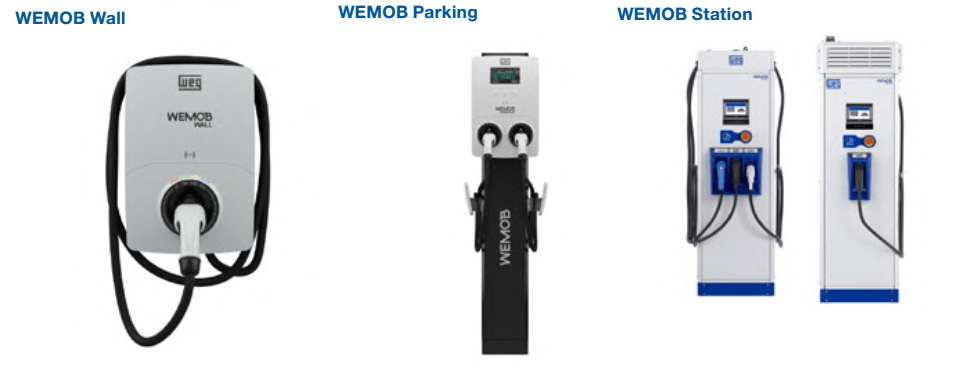
\includegraphics[width=0.95\textwidth]{./Figuras/etacoes_recarga.png}
    \caption{Estação de recarga lenta, rápida e ultrarrápida respectivamente.}{Fonte: \cite{weg_estacao}}
   \label{fig:etacoes_recarga}
\end{figure}

\end{frame}

%--------------------

\begin{frame}{Estação de recarga tipos de conectores}

\begin{figure}[H]
    \centering
    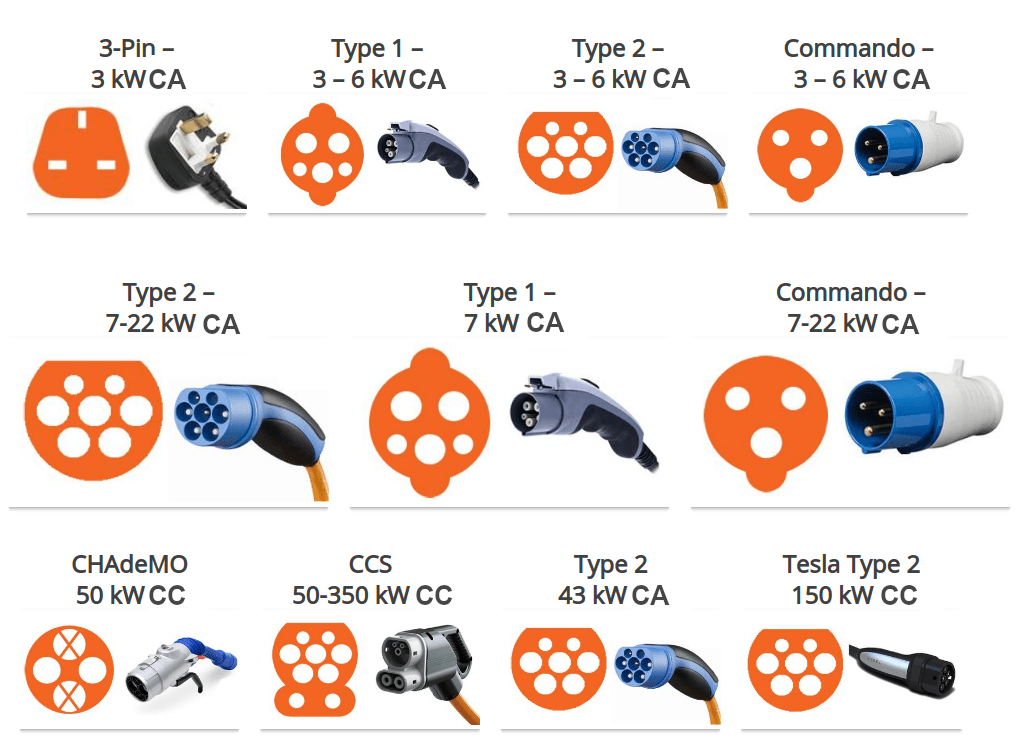
\includegraphics[width=0.7\textwidth]{./Figuras/chargers.png}
    \caption{Tipos de conectores usados nas estações de recarga.}{Fonte: \cite{ev_conect_zap}}
   \label{fig:fast_chargers}
\end{figure}

\end{frame}

%--------------------

\begin{frame}{Estruturas para painéis fotovoltaicos}

\begin{figure}[H]
    \centering
    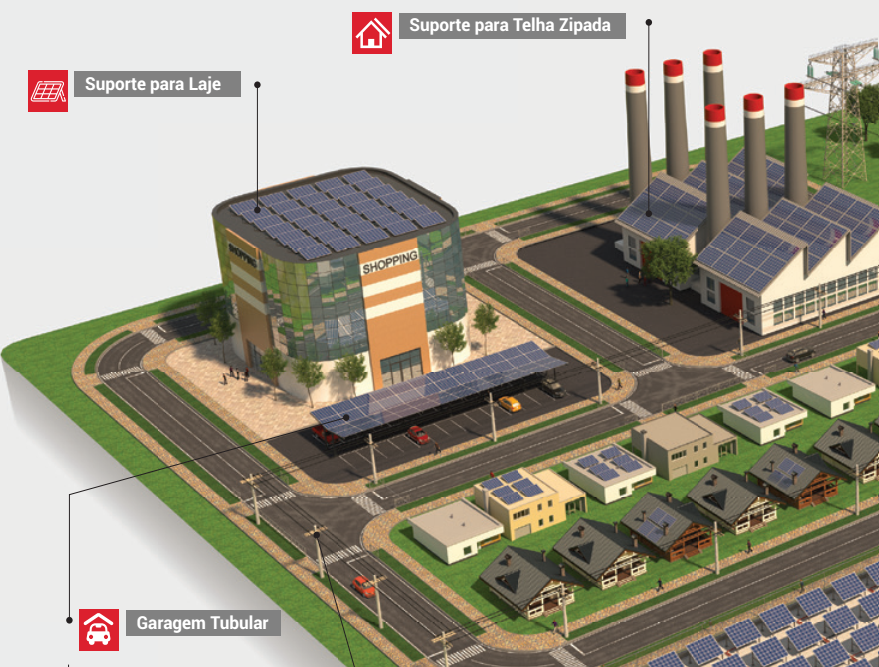
\includegraphics[width=0.65\textwidth]{./Figuras/estruturas.png}
    \caption{Estruturas para painéis fotovoltaicos.}{Fonte: \cite{romagnole}}
   \label{fig:estruturas}
\end{figure}


\end{frame}

%--------------------

\begin{frame}{Resumo financeiro}

\scriptsize
\begin{table}[htbp]
    \caption{Resumo custos pesquisados}
        \begin{center}
            \begin{tabular}{ >{\centering\arraybackslash} m{4cm} >{\centering\arraybackslash} m{2cm} >{\centering\arraybackslash} m{3cm}  }
                \hline
                Tipo & Custo  R\$ &  Observação \\ \hline %Primeira e ultima linha adiciona \hline apos \\
                kWh & 0,83 a 0,92  & Por kWh consumido \\
                Painéis (PV) & 2,2 a 2,35 & Por Wp \\
                Inversores (CC CA) & 150 a 750 & Por kW de potencia de inversão\\
                Otimizador de potência  & 250 a 600  & Cada unidade \\
                Microinversor & 750 a 1500  & Por conexão de painel \\
                Estrutura para veículos  & 5 a 15 mil  & Por vaga \\
                Estrutura para laje concreto  & 150 a 500  & Por painel \\
                Estrutura para telhas  & 50 a 320  & Por painel \\
                Carregadores ultrarrápidos  & 40 a 100 mil  & Por unidade \\
                Carregadores rápidos  & 27 a 35 mil  & Por unidade \\
                Carregadores lentos  & 7,5 a 10 mil  & Por unidade \\ \hline
            \end{tabular}
        \end{center}
    \label{resumo}
\end{table}

\end{frame}

%--------------------

\begin{frame}{Modelo financeiros custos e retornos}

Com base na tabela \ref{resumo} foi desenvolvido um modelo capaz de determinar os custos e retornos financeiros. Neste modelo temos equações para calcular:

\begin{itemize}
  \item Retorno estações de recarga.
  
  \item Custo total estações de recarga.

  \item Custo total do sistema PV.
  
  \item Consumo total de energia ano.
  
  \item Déficit/Excedente de energia ano.
  
   \item Custo total do sistema.
   
   \item Retorno total do sistema ano.
   
   \item Lucro anual apos sistema pago
   
   \item Etc...
\end{itemize}

\end{frame}

%--------------------

\begin{frame}{As linguagens usadas no sistema}

\begin{itemize}

  \item \textbf{JavaScript} usada para desenvolver a lógica de programação para WEB.
  
  \item \textbf{HTML} usada para criar a estrutura visual os documentos que compõem o aplicativo.

  \item \textbf{CSS} usada para definir os estilos dos documentos HTML do aplicativo.
  
\end{itemize}

\end{frame}

%--------------------

\begin{frame}{O banco de dados}

Os dados possíveis de calcular são gerados usando a biblioteca \textit{pvlib python} disponível no site \url{https://pvlib-python.readthedocs.io} desenvolvida por \cite{pvlib}, com esta é possível obter para uma região qualquer por exemplo: 

\begin{itemize}

  \item Posição geográfica solar.
  
  \item Ângulo de incidência (AOI).

  \item Ângulo azimute $\theta_A$.
  
  \item Ângulo zênite $\theta_Z$.
  
\end{itemize}

Python é uma linguagem de programação interpretada, orientada a objetos e de alto nível com tipagem dinâmica.

\end{frame}

%--------------------

\begin{frame}{Dados obtidos pvlib}

\begin{figure}[H]
    \centering
    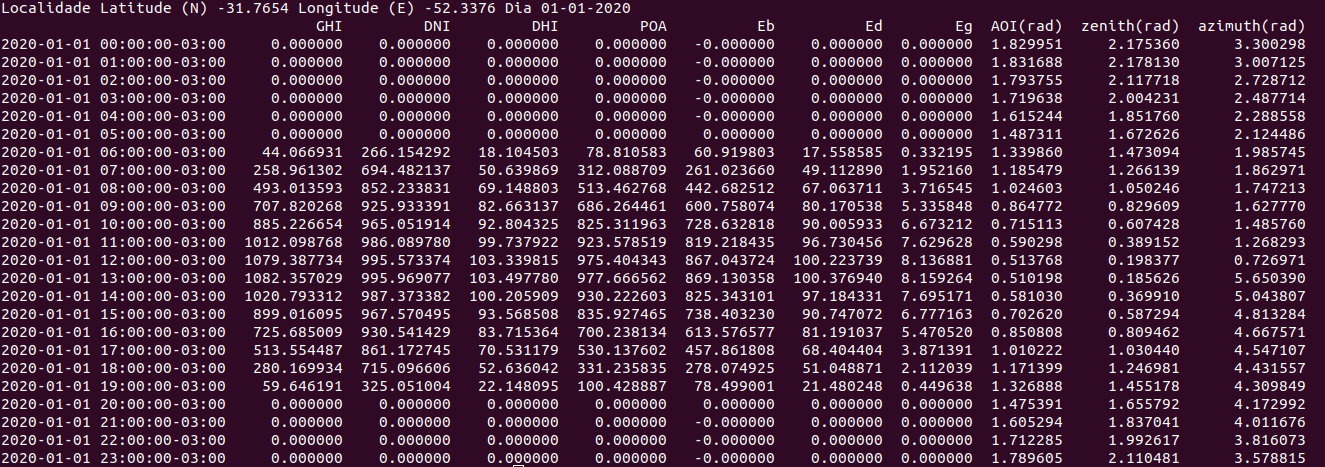
\includegraphics[width=1\textwidth]{./Figuras/pv_lib_pelotas_dados.png}
    \caption{Dados obtidos usando a biblioteca pvlib, para um dia de verão de Pelotas.}
   \label{fig:pv_lib_pelotas_dados}
\end{figure}

\end{frame}

%--------------------

\begin{frame}{O banco de dados}

Os dados não possível de calcular são fornecidos pelo site \url{https://pvwatts.nrel.gov/pvwatts.php} este contempla uma serie de informações de estações do mundo todo, no Brasil temos dados de estações em todas regiões, dentro destas informações temos os dados divididos por, Mês, Dia e Hora que contem:

\begin{itemize}

  \item Irradiância solar (W/m²).
  
  \item Temperatura ambiente (°C).

  \item Velocidade do vento (m/s).

\end{itemize}

\end{frame}

%--------------------

 %============================================================
\section{Resultados}
\begin{frame}{Resultados}
Foi escolhido dois locais reais para usar como referencia para obter os resultados, o ShoppingPelotas uma residência.

\begin{figure}[H]
    \centering
    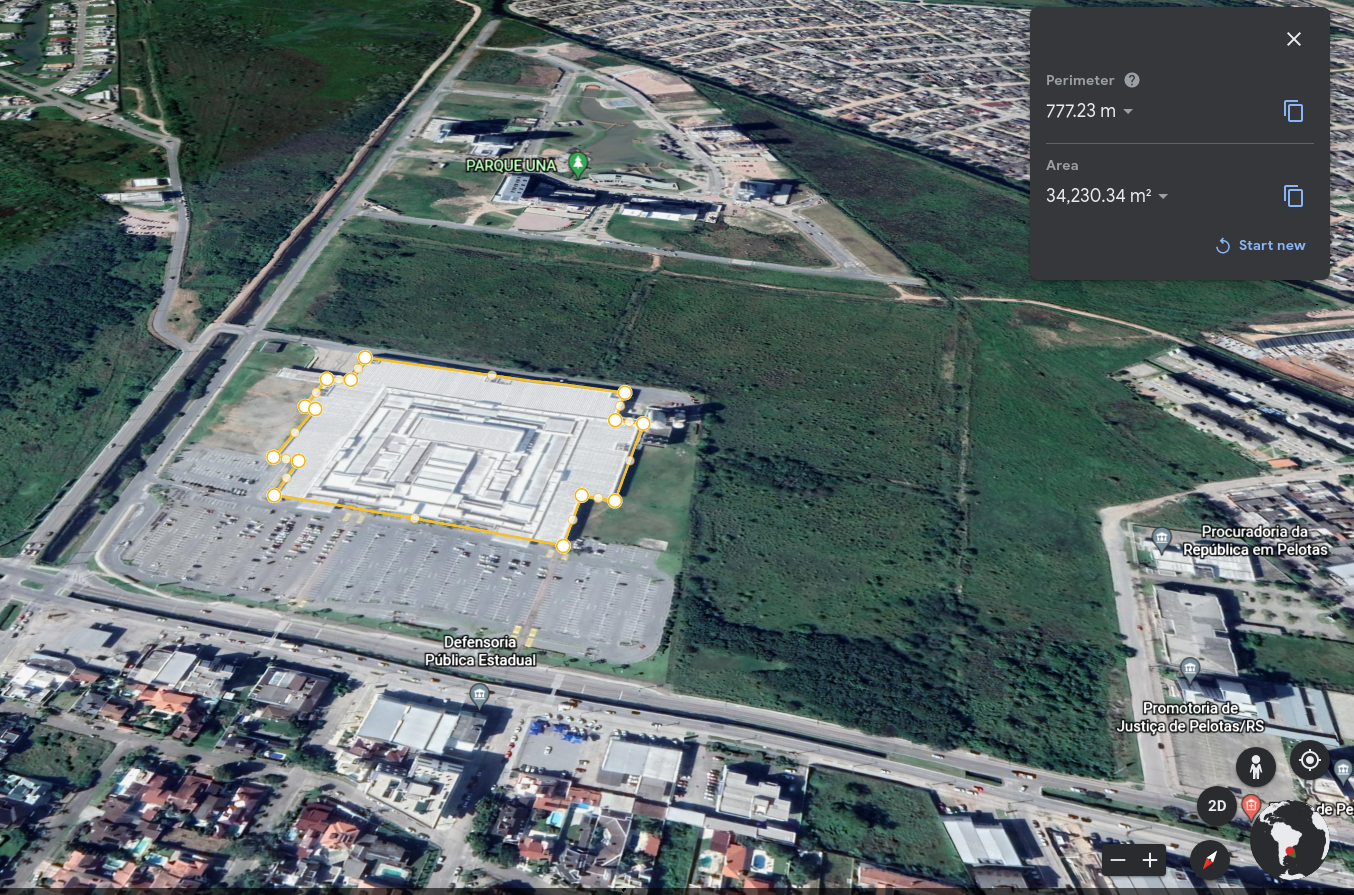
\includegraphics[width=0.65\textwidth]{./Figuras/shopping_1.png}
    \caption{Área cobertura Shopping.}
   \label{fig:shopping_1}
\end{figure}

\end{frame}
%-----------------------------

%============================================================
\begin{frame}

\begin{figure}[H]
    \centering
    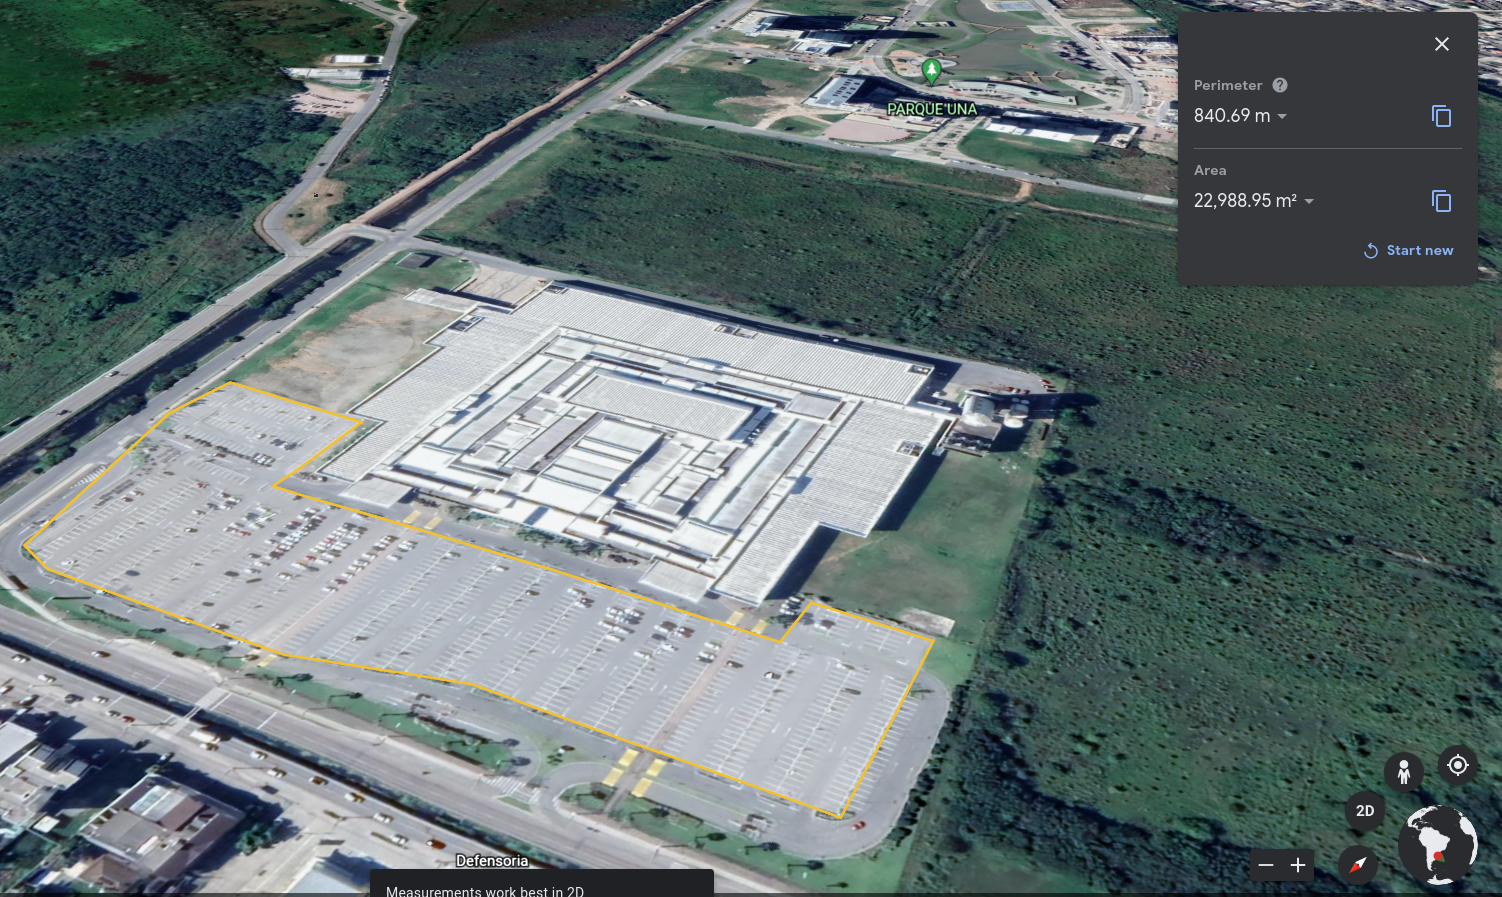
\includegraphics[width=0.95\textwidth]{./Figuras/shopping_2.png}
    \caption{Área estacionamento Shopping.}
   \label{fig:shopping_2}
\end{figure}

\end{frame}
%-----------------------------

%============================================================
\begin{frame}

\begin{figure}[H]
    \centering
    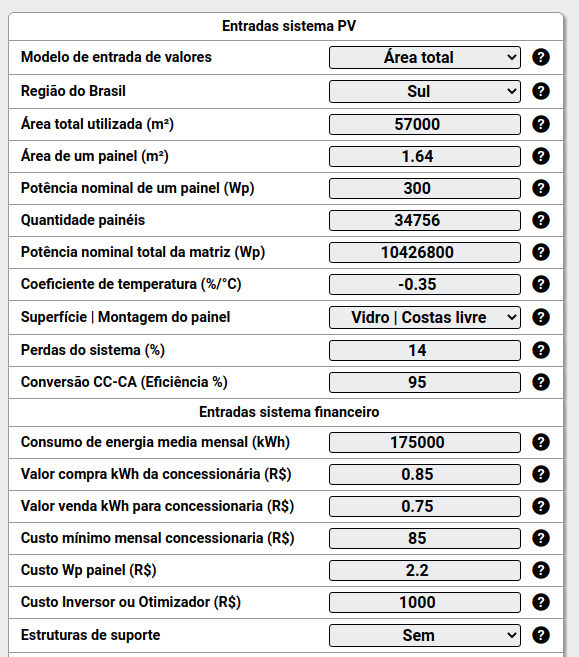
\includegraphics[width=0.5\textwidth]{./Figuras/shopping_3.png}
    \caption{Shopping Pelotas produção de energia total anual entrada.}
   \label{fig:shopping_3}
\end{figure}

\end{frame}
%-----------------------------

%============================================================
\begin{frame}

\begin{figure}[H]
    \centering
    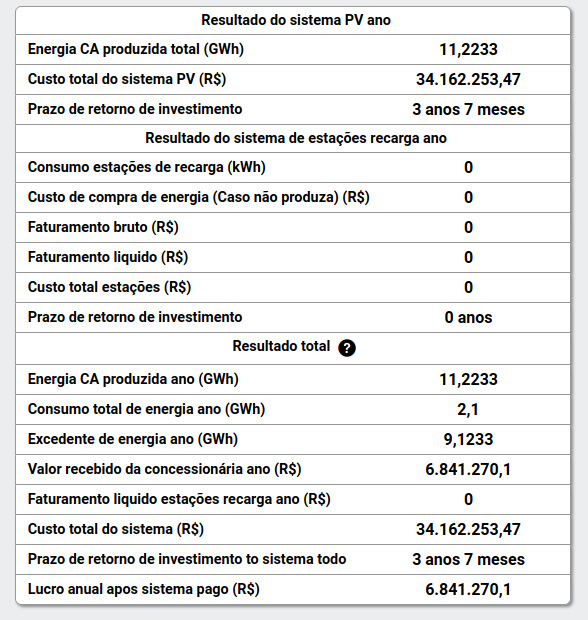
\includegraphics[width=0.5\textwidth]{./Figuras/shopping_4.png}
    \caption{Shopping Pelotas produção de energia total anual resultado.}
   \label{fig:shopping_4}
\end{figure}

\end{frame}
%-----------------------------

%============================================================
\begin{frame}

\begin{figure}[H]
    \centering
    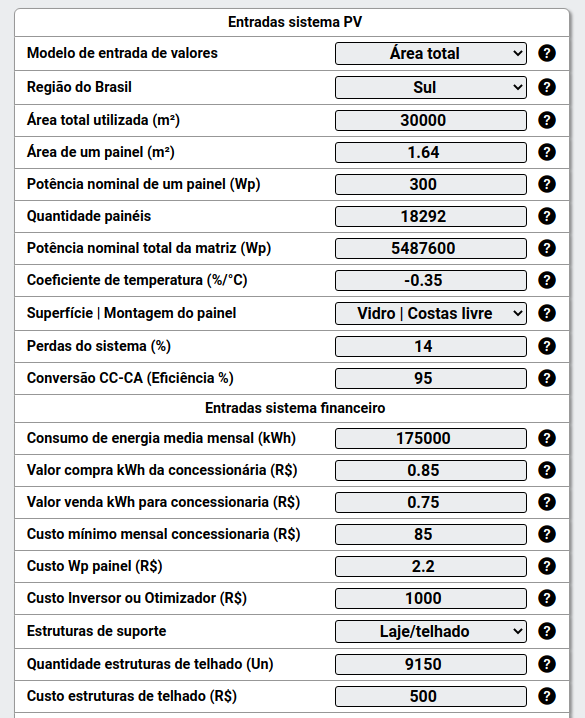
\includegraphics[width=0.5\textwidth]{./Figuras/shopping_5_1.png}
    \caption{Entradas da estimativa do shopping como estação de recarga e cogeração de energia.}
   \label{fig:shopping_5_1}
\end{figure}


\end{frame}
%-----------------------------

%============================================================
\begin{frame}

\begin{figure}[H]
    \centering
    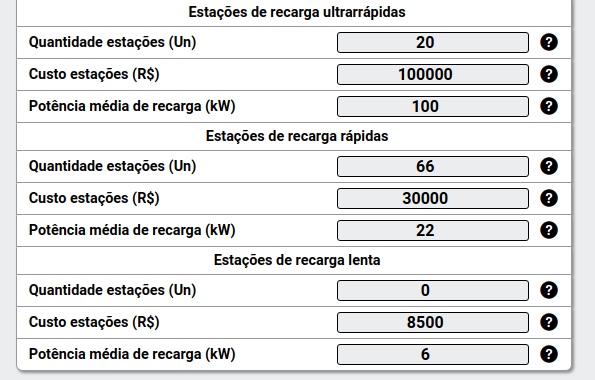
\includegraphics[width=0.5\textwidth]{./Figuras/shopping_5_2.png}
    \caption{Entradas da estimativa do shopping como estação de recarga e cogeração de energia.}
   \label{fig:shopping_5_2}
\end{figure}


\end{frame}
%-----------------------------

%============================================================
\begin{frame}


\begin{figure}[H]
    \centering
    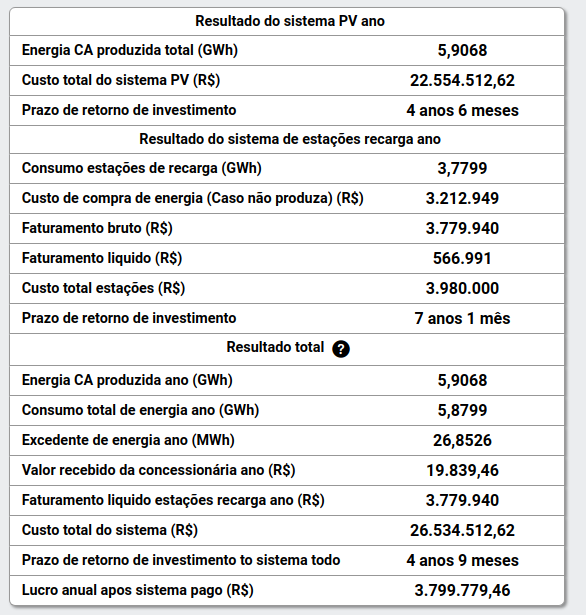
\includegraphics[width=0.5\textwidth]{./Figuras/shopping_6.png}
    \caption{Resultado da estimativa do shopping como estação de recarga e cogeração de energia.}
   \label{fig:shopping_6}
\end{figure}

\end{frame}
%-----------------------------

%============================================================
\begin{frame}

\begin{figure}[H]
    \centering
    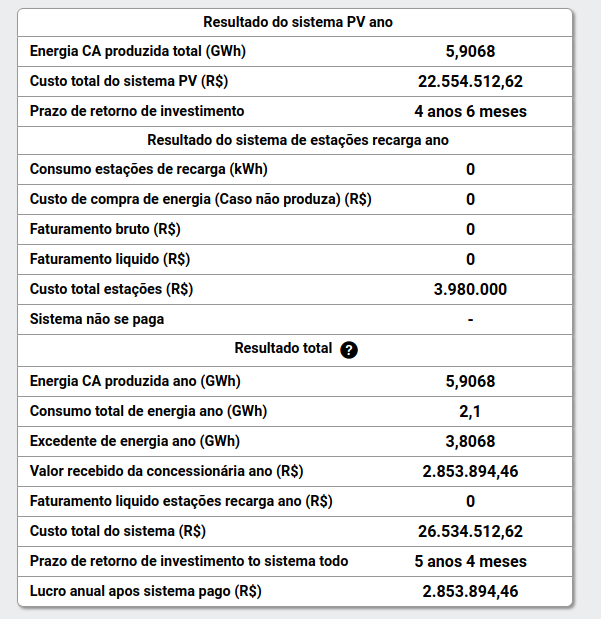
\includegraphics[width=0.5\textwidth]{./Figuras/shopping_7.png}
    \caption{Resultado da estimativa do shopping como estação de recarga e cogeração de energia, trafego veículos elétricos zero.}
   \label{fig:shopping_7}

\end{figure}
\end{frame}
%-----------------------------

%============================================================
\begin{frame}

\begin{figure}[H]
    \centering
    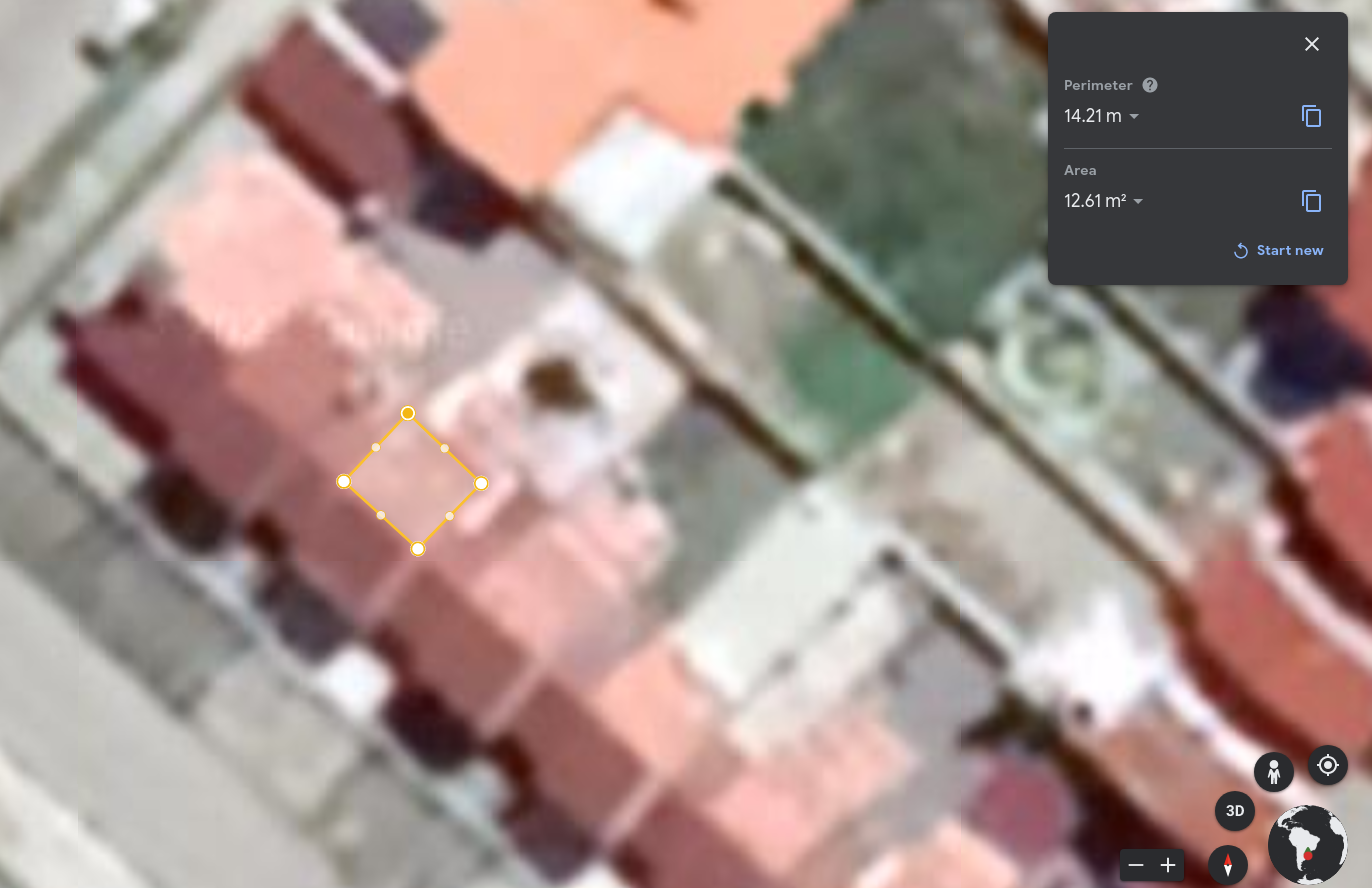
\includegraphics[width=0.95\textwidth]{./Figuras/casa_minha.png}
    \caption{Residencia telhado de 40 m² na cidade de pelotas.}
   \label{fig:casa_minha}
\end{figure}

\end{frame}
%-----------------------------

%============================================================
\begin{frame}

\begin{figure}[H]
    \centering
    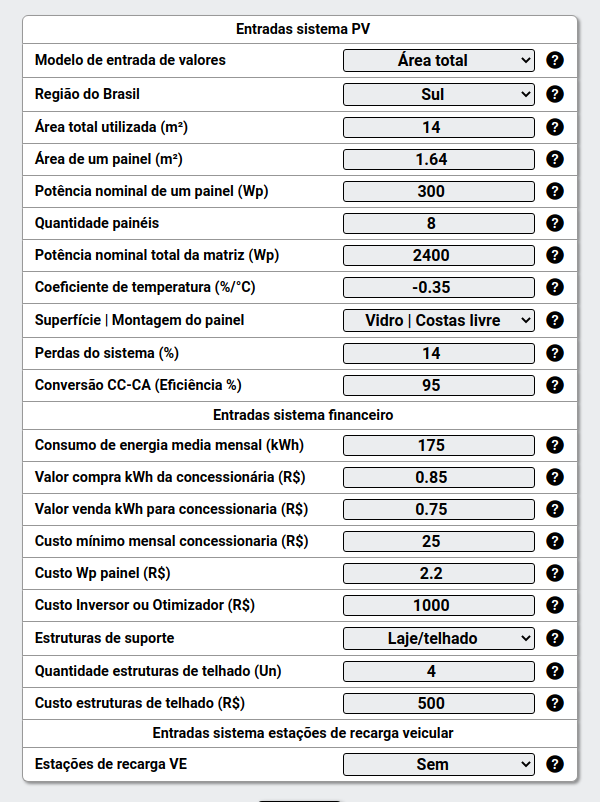
\includegraphics[width=0.5\textwidth]{./Figuras/casa_minha_1.png}
    \caption{Entradas sistema PV para uma residência com telhado de 40 m² na cidade de Pelotas.}
   \label{fig:casa_minha_1}
\end{figure}

\end{frame}
%-----------------------------

%============================================================
\begin{frame}

\begin{figure}[H]
    \centering
    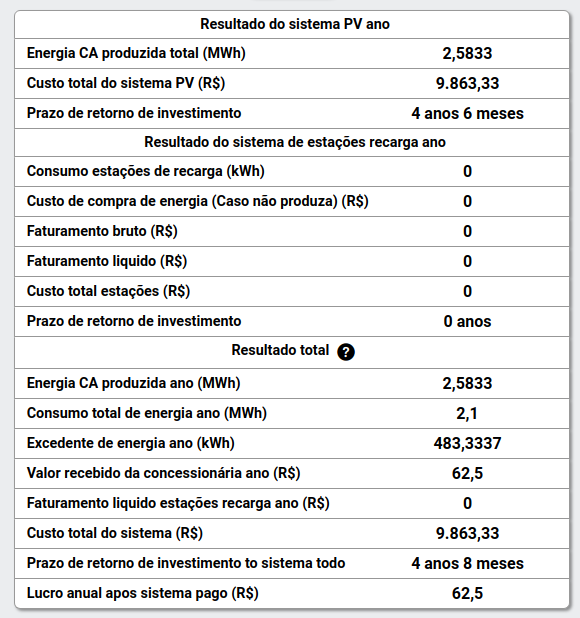
\includegraphics[width=0.5\textwidth]{./Figuras/casa_minha_1_2.png}
    \caption{Resultado para uma residência com telhado de 40 m² na cidade de Pelotas.}
   \label{fig:casa_minha_1_2}
\end{figure}

\end{frame}
%-----------------------------
\begin{frame}

\begin{table}[htbp]
    \caption{Comparativo autonomia veículos elétrico e gasolina}
        \begin{center}
            \begin{tabular}{ >{\centering\arraybackslash} m{3cm} >{\centering\arraybackslash} m{3cm} >{\centering\arraybackslash} m{3cm}  }
                \hline
                Tipo & Distância &  Custo \\ \hline %Primeira e ultima linha adiciona \hline apos \\
                Elétrico & 15 Km & R\$  2,60 (3 kWh) \\
                Gasolina & 15 Km & R\$ 7 (1 Litro)\\ \hline
            \end{tabular}
        \end{center}
    \label{ev_gas}
\end{table}

\end{frame}

%============================================================
\begin{frame}


\begin{figure}[H]
    \centering
    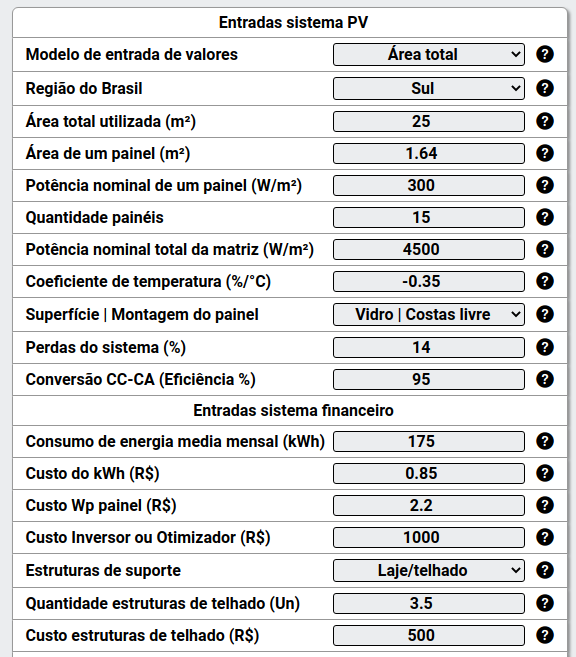
\includegraphics[width=0.525\textwidth]{./Figuras/casa_minha_2.png}
    \caption{Entradas sistema PV para uma residência com telhado de 40 m² na cidade de Pelotas.}
   \label{fig:casa_minha_2_1}
\end{figure}

\end{frame}
%-----------------------------

%============================================================
\begin{frame}


\begin{figure}[H]
    \centering
    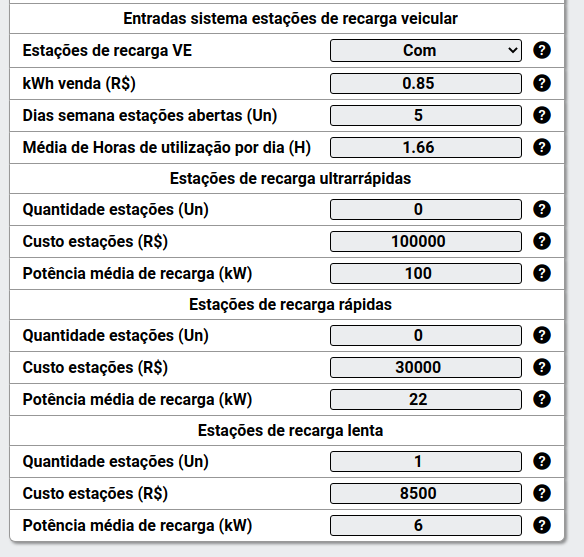
\includegraphics[width=0.6\textwidth]{./Figuras/casa_minha_2_2.png}
    \caption{Entradas estações de recarga para uma residência com telhado de 40 m² na cidade de Pelotas.}
   \label{fig:casa_minha_2_2}
\end{figure}

\end{frame}
%-----------------------------
%============================================================
\begin{frame}


\begin{figure}[H]
    \centering
    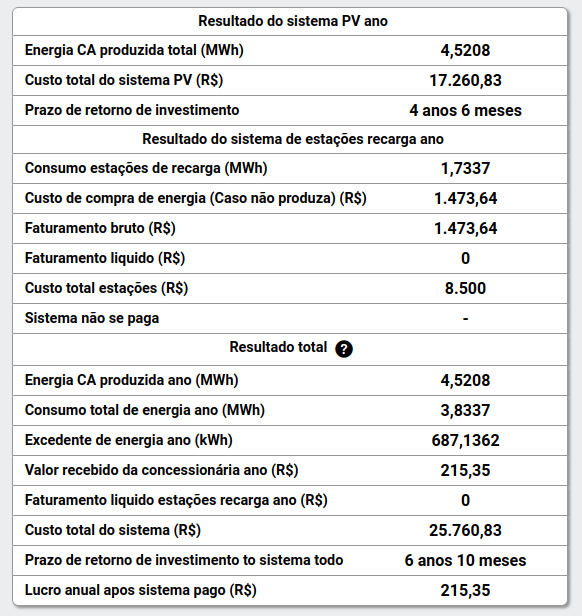
\includegraphics[width=0.5\textwidth]{./Figuras/casa_minha_2_3.png}
    \caption{Resultado para uma residência com telhado de 40 m² na cidade de Pelotas.}
   \label{fig:casa_minha_2_3}
\end{figure}

\end{frame}
%-----------------------------

%===============================================================
\section{Conclusão}

\begin{frame}{Conclusão}

\Large
\centering
    
\textbf{Conclusão}

\textbf{e}

\textbf{Trabalhos futuros}

\end{frame}

\section{Referências bibliográficas}
\begin{frame}[allowframebreaks]
        \printbibliography[heading=none]
\end{frame}

%--------------------------------

\end{document}